\documentclass[a4paper,12pt]{book}

\usepackage{natbib}
\usepackage{amsmath}
\usepackage[pdftex]{graphicx}
\usepackage{array}
\usepackage{moreverb}
\usepackage{color}
\usepackage[plainpages=false,pdfpagelabels]{hyperref}
\usepackage{url}
% new color
\definecolor{mylinkcolor}{rgb}{0,0,0.75}
\definecolor{mycitecolor}{rgb}{0,0.5,0}
\definecolor{myfilecolor}{rgb}{1,0,0}
\definecolor{myurlcolor}{rgb}{0.25,0.5,0.25}
\hypersetup{
bookmarks=true,         % show bookmarks bar?
pdftoolbar=true,        % show Acrobat’s toolbar?
pdfmenubar=true,        % show Acrobat’s menu?
pdffitwindow=true,       % page fit to window when opened
colorlinks=true,        % false: boxed links; true: colored links
linkcolor=mylinkcolor,  % color of internal links
citecolor=mycitecolor,  % color of links to bibliography
filecolor=myfilecolor,    % color of file links
urlcolor=myurlcolor     % color of external links
}

\usepackage[all]{hypcap}
\usepackage{courier}

% Version number
\newcommand{\Version}{0.6.4d}

% layout
\setlength\topmargin{0in}
\setlength\headheight{0in}
\setlength\headsep{1in}
\setlength\textheight{7.7in}
\setlength\textwidth{6.5in}
\setlength\oddsidemargin{0in}
\setlength\evensidemargin{0in}
\pagestyle{headings}

% Set that there is no numbering for chapters, parts, sections, etc.
\setcounter{secnumdepth}{2}
% Set that there is a table of contents for all.
\setcounter{tocdepth}{2}

% MACROS
\newcommand{\TT}[1]{{\tt #1}} % typewriter typeface
\newcommand{\BF}[1]{{\bf #1}} % bold
\newcommand{\IF}[1]{{\it #1}} % italic
\newcommand{\QU}[1]{``#1''} % strict quotation marks
\newenvironment{script}{\\\\\footnotesize\$\TT}{\normalsize\\\\}
% Short forms for names
\newcommand{\rGFF}{reference genome FASTA file} 
\newcommand{\RGFF}{Reference genome FASTA file} 
\newcommand{\rFF}{reads FASTQ file}
\newcommand{\RFF}{Reads FASTQ file}
\newcommand{\BRGF}{BFAST reference genome file} % short form for brg
\newcommand{\BIF}{BFAST index file} % short form for bif
\newcommand{\BMF}{BFAST matches file} % short form for bmf
\newcommand{\BAF}{BFAST aligned file} % short form for baf
%\newcommand{\BMAF}{BFAST multiple sequence alignment file} % short form for the bfast output (maf)
%\newcommand{\BGFFF}{BFAST general feature format file} % short form for the bfast output (gff)
\newcommand{\BSAMF}{BFAST sequence alignment/map file} % short for for the bfast output (sam) 
\newcommand{\FIVETOTHREE}{$5'\rightarrow3'$} % 5 prime to 3 prime

% DATE
\author{Nils Homer}
\date{}
\title{BFAST: BLAT-like Fast Accurate Search Tool
\thanks{Copyright \copyright\ UCLA 2008, made for BFAST version \Version}
}
\begin{document}
\frontmatter

% TITLE PAGE
%\thispagestyle{empty} % Suppress page numberings on the first page
\maketitle

% TABLE OF CONTENTS
\tableofcontents
\addcontentsline{toc}{chapter}{Table of Contents}

\listoffigures
\addcontentsline{toc}{chapter}{List of Figures}
\listoftables
\addcontentsline{toc}{chapter}{List of Tables}

\chapter{Preface}
This document is meant to serve as a guide for the practical use of BFAST.
It includes explanations of all command-line options for each command and binary in BFAST to give an idea of basic usage.
Input and output file formats are also detailed.
We give many examples of use, including alignment to the whole genome, targeted genomic regions, and to the transcriptome.

This document does not try to explain the underlying algorithm or data-structures used in BFAST.
For example, we will not explain the local alignment algorithms, or the underlying BFAST algorithm.
Without proper understanding of the underlying algorithm, including local alignment algorithms, it is difficult to use this very flexible program knowledgeably to obtain your desired results.
Therefore, reading the BFAST paper (\cite{BFAST}) is a strict prerequisite.
Additionally, the local alignment paper used by BFAST for ABI SOLiD data is required for ABI SOLiD data alignment (\cite{BFAST-local-alignment}).

If you have anything that you would be useful to add to this guide, feel free to relay the addition to the BFAST developers.
This includes but is not limited to bugs, typos, and explanations.
Please see \url{http://genome.ucla.edu/bfast} for more details.

Enjoy!

\section{Acknowledgements}
We would like to thank Jim Kent for creating and distributing the BLAT program (\cite{BLAT}), which was both a motivation for this work, and was also the basis for our initial practical large scale alignment pipeline.
We also thank members of the Nelson Lab: Zugen Chen, Hane Lee, Bret Harry, Jordan Mendler, Brian O’Connor for input and computational infrastructure support.

The layout and organization of this book was guided by the design found in the SVN book (\url{http://svnbook.red-bean.com/}).
We would also like to thank SVN for creating amazing version control software that manages the source code BFAST.
\mainmatter

\chapter{Run BFAST now!}
So impatient!
If you want to run BFAST now, you have come to the right place.
If you are aligning Illumina data or ABI SOLiD data to the human genome, please see \autoref{sec:hg-settings}.  
Otherwise, then please check out the High Speed Tutorial (\autoref{sec:high-speed-tutorial}).

\chapter{Fundamental Concepts}
\section{What is BFAST?}
The short answer is that BFAST is a tool for fast and accurate sequence alignment (it is in the name).
An implementation of BFAST can be found at \url{http://bfast.sourceforge.net}.
The longer answer is, well, longer.

The basic problem is as follows.
We are given some reference sequence, to which we wish to compare our data.
Our data are short reads (sometimes numbering in the billions) that are substrings of the reference sequence.
In some cases, these short reads differ based on various edit operators that modify the read in some fashion.
It is the goal of BFAST to find the location in the reference sequence that minimizes the number of edit operators used to transform the read into the reference sequence at that location.
The process of concluding a read has a location in the reference sequence is called mapping or alignment.

In the case of DNA sequence alignment, these edit operators are biologically and technology motivated, including mutations/mismatches/SNPs, insertion of bases (or letters), deletion of bases (or letters), and technical errors. 
Typically we have some set of sequence to which we wish to compare our reads.
In many cases, finding the correct location given a set of variants (such as the operators) is extremely important since we may be only interested in the variants themselves.

For example, we may be interested in mutations in Breast Cancer and therefore mapping accurately or robust to many combinations of variants is important.
In other cases, the speed of mapping is important and the accuracy is not. 
For example, in digital gene expression analysis the goal is to estimate the number of reads map over locations in the genome as to gain an overall trend of coverage, rather than precise variant detection.

Whatever is the intended application of BFAST, it can be tuned to find alignments quickly at the cost of accuracy or robustness against variants.
It can also be tuned to accurately find alignments with variants at the cost of speed. 
This is the power of BFAST.
It is a highly generalized algorithm allowing the user to tune the algorithm to suit their specific needs.

Its implementation is ever-evolving, with new releases occurring early in development and often. 
BFAST is suited for use on high memory machines when used for Human Genome resequencing and is best used on a cluster of such machines.
Nevertheless, it is able to be efficiently run on low memory machines (<4GB) even for the Human Genome.
It also uses multi-threaded programming to utilize the multi-core architecture of current machines.
The output of BFAST is in binary format to reduce file space for large data, although we supply tools to convert these formats to text or other standard formats if so desired.
Finally, we use the \TT{C} programming language to implement BFAST to increase efficiency as well as the GNU Build System (Autotools) to handle compilation.

\section{Program Organization}
BFAST consists of two sets of programs.
The most important utilities are combined into one program \TT{bfast}.  
A command is specified this one binary to run each command.
Auxiliary commands are separated into their own individual programs in the \TT{butil} folder.

\section{Work flow}
\label{sec:work-flow}
The basic work flow has five steps as seen in \autoref{fig:work-flow}.
\begin{figure}[t]
	\centering
	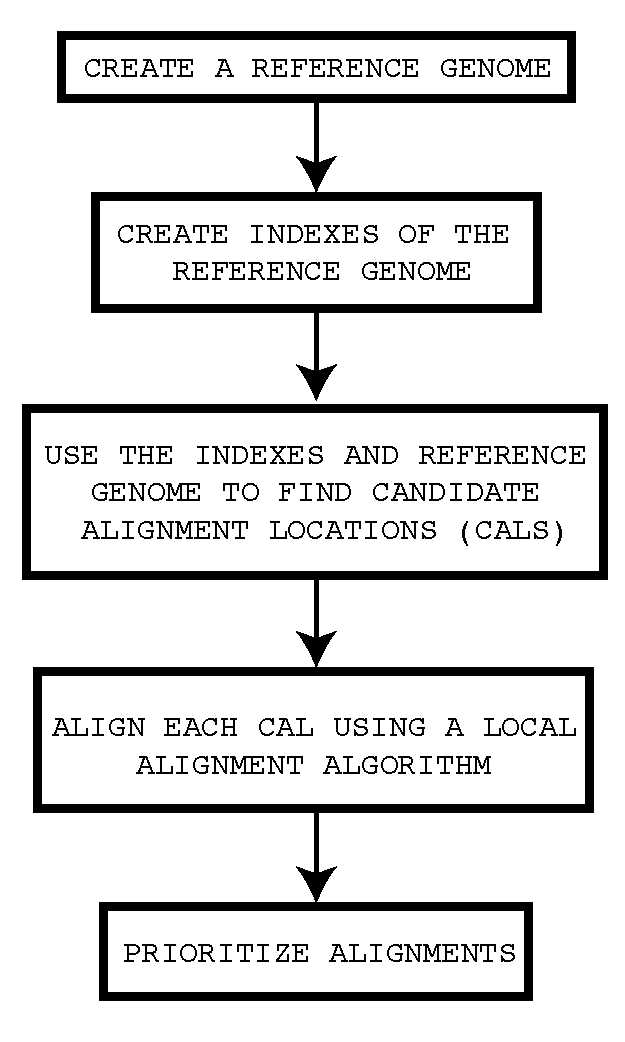
\includegraphics[scale=0.75]{work-flow.pdf}
	\caption{
	The BFAST work flow.
	}{
	See \autoref{sec:work-flow} for a description.
	\label{fig:work-flow}
	}
\end{figure}

\begin{enumerate}
	\item
		The first step is to create a reference genome.
		This reference genome contains all the sequence to which we wish to align.
		The command \TT{bfast fasta2brg} performs this task (see \autoref{sec:fasta2brg}).
	\item
		The second step is to create indexes of the reference genome, which was created in the first step.
		The number and layout of these indexes is determined both by the user's speed and accuracy requirements.
		The command \TT{bfast index} performs this task (see \autoref{sec:index}).
	\item
		The third step is to find candidate alignment locations (CALs) for each read.
		The expected number of CALs returned is a function of the number of indexes and the layouts chosen in the second step as well as the number offsets.
		The binary \TT{bfast match} performs this task (see \autoref{sec:match}).
	\item
		The fourth step is to fully align each CAL for each read.
		This uses a standard local alignment algorithm (\cite{SmithWaterman}) or a custom tool for ABI SOLiD data (\cite{BFAST-local-alignment}).
		The binary \TT{bfast localalign} performs this task (see \autoref{sec:localalign}).
	\item
		The fifth and final step is to prioritize the final alignments.
		The user specifies criteria to select the correct alignment for each read.
		The criteria can be based on many factors, including uniqueness, score, or other factors.
		The binary \TT{bfast postprocess} performs this task (see \autoref{sec:postprocess}).
\end{enumerate}

The reference genome (Step 1) and indexes (Step 2) can be re-used between experiments where only the read data changes, not the reference genome or index layouts.
Since only the reads will change, one can utilize the same reference genome and indexes created in Step 1 and Step 2 respectively.
Therefore, it is advised to perform Step 1 and Step 2 such that the reference genome and indexes can be re-used, thus reducing the work flow down to three steps upon re-use.
In fact, the main speed of this program comes from the idea that in general, the reference genome and associated indexes need only be built once, with the reads coming from the same reference genome (say Human) but different samples or experiments.

\chapter{Basic Usage}
BFAST is a command-line program.
It accepts many command-line options to customize and tune the alignment algorithm.
The key commands are organized into one binary program called \TT{bfast}.
To access each command, we use \TT{bfast <command>}.
As seen in the \autoref{sec:work-flow}, there are five commands to be run for the entire work flow, although only three need to be used if we are aligning to the same reference genome using the same indexes.
\section{Common Options}
\label{sec:commonoptions}
Some common options exist across some or all of the commands. 

These options include specifying the reference genome FASTA file, specifying the number of threads for parallel processing (\TT{-n}), the number of reads to load at a time (\TT{-Q}), specifying where temporary files should be stored (\TT{-T}), specifying the encoding space (\TT{-A}), outputting timing information (\TT{-t}), printing program parameters (\TT{-p}), and printing a help message (\TT{-h}).

Other options, such as the options \TT{-s}, \TT{-S}, \TT{-e}, and \TT{-E} for specifying only a contiguous range should be considered, are shared across some of the commands but have specific implications to each command and are described in the respective command's section.

The BFAST commands \TT{match}, \TT{localalign}, and \TT{postprocess} can all accept their input file from the standard input stream, facilitating the use of these BFAST commands in a pipe-and-filter model.
For example, this allows the output of \TT{match} to be piped into \TT{localalign}, with the subsequent output be piped into \TT{postprocess}. 
When the input for these commands comes from the standard input stream, no progress messages of any kind will be outputted (don't panic).

\subsection{Usage}
\subsubsection{\TT{-f FILENAME, --fastaFileName=FILENAME}}
Specifies the file name of the FASTA reference genome (see \autoref{sec:rgfastafile} for the file format).
This option applies to \TT{bfast fasta2brg}, \TT{bfast index}, \TT{bfast match}, \TT{bfast localalign}, and \TT{bfast postprocess}.
\subsubsection{\TT{-n INTEGER, --numThreads=INTEGER}}
For \TT{bfast index} the number of threads must be a power of two due the implementation of the index sorting algorithm (merge sort).
Otherwise it is recommended that the number of threads match the number of cores or processors.
This option applies to \TT{bfast index}, \TT{bfast match}, \TT{bfast localalign}, and \TT{bfast postprocess}. 

\subsubsection{\TT{-Q INTEGER, --queueLength=INTEGER}}
Specifies the number of reads to cache or load into memory at one time.
This option applies to \TT{bfast match}, \TT{bfast localalign}, and \TT{bfast postprocess}.

\subsubsection{\TT{-T DIRECTORY --tmpDir=DIRECTORY}}
This option specifies the directory in which to store temporary files.
For large datasets, the necessary disk space for temporary files may be large and therefore it is useful to to specify the temporary file directory. 
Be sure to include a trailing backslash or $\backslash$.
If no option is given, the temporary file directory is defaulted to the current directory.
This option applies to \TT{bfast index}, and \TT{bfast match}.

\subsubsection{\TT{-A INTEGER, --space=INTEGER}}
Specifies the encoding space of the alphabet.
For nucleotide space, use \TT{-A 0} (Illumina, 454, etc.).
For color space, use \TT{-A 1} (ABI SOLiD).

\subsubsection{\TT{-t, --timing}}
This option applies to \TT{bfast fasta2brg}, \TT{bfast index}, \TT{bfast match}, \TT{bfast localalign}, and \TT{bfast postprocess}.
This option causes timing information for the execution of the program to be displayed upon successful termination.

\subsubsection{\TT{-p, --Parameters}}
This option applies to \TT{bfast fasta2brg}, \TT{bfast index}, \TT{bfast match}, \TT{bfast localalign}, and \TT{bfast postprocess}.
This option causes the input command-line parameters to be displayed and subsequent termination of the program.

\subsubsection{\TT{-h, --Help}}
This option applies to \TT{bfast fasta2brg}, \TT{bfast index}, \TT{bfast match}, \TT{bfast localalign}, and \TT{bfast postprocess}.
This option prints a help message.

\section{bfast fasta2brg}
\label{sec:fasta2brg}
\BF{fasta2brg} is a command that is used to create a reference genome from FASTA file.
This utility performs the first step of the work flow outlined in \autoref{sec:work-flow}.
The \BRGF{} will be written in compressed binary format to preserve space.
See \autoref{sec:brgf} for the file format of the \BRGF{}.

See \autoref{sec:commonoptions} for common options that are in use in this command.
\subsection{Creating a Reference Genome}
\label{sec:creating-a-rg}
To create a reference genome, the required command-line options is \TT{-f}.

We need to input a \rGFF{} using the \TT{-f} option (see \autoref{sec:rgfastafile} for the file format).
To create a reference genome in color space, we use the option \TT{-A 1}, otherwise we use \TT{-A 0}.

When creating a \BRGF{}, the contigs will be numbered according to their order in the \rGFF{} (option \TT{-f}).
The numbering is one-based (begins with one).
The maximum number of contigs is $2^{31}$ or $2147483648$.
The name of each contig specified in the header of the \rGFF{} will be also be stored.
The maximum sequence length for a single contig is also $2^{31}$ or $2147483648$. 
The input sequence will be assumed to be the forward strand of the genome.
Only the forward strand of the genome will be stored (see \autoref{sec:brgf} for more details).
The output will be a \BRGF{} (see \autoref{sec:brgf} for the file format).

\section{bfast index}
\label{sec:index}
\BF{index} is a command that is used to create the indexes of a reference genome.
This utility performs the second step of the work flow outlined in \autoref{sec:work-flow}.
The \BIF{} will be written in compressed binary format to preserve space.
See \autoref{sec:bif} for the file format of the \BIF{}.

See \autoref{sec:commonoptions} for common options that are in use in this command.
\subsection{Creating Indexes of a Reference Genome}
\label{sec:creating-bifs}
To create indexes of a reference genome, the required command-line options are \TT{-f}, \TT{-m}, and \TT{-w}.

We need to input a \rGFF{} using the \TT{-f} option (see \autoref{sec:rgfastafile} for the file format).
The \BRGF{} must already be created using this \rGFF{} using \TT{bfast fasta2brg} and will be inferred from the \rGFF{} file name.
If we choose to create the indexes in color space (\TT{-A 1}), a color space \BRGF{} must exist.
The \TT{-m} option specifies the mask or space-seed to use for this index.
The \TT{-w} option specifies the hash width (the index into the index).

The \TT{-d} option is used to split the index into multiple parts for low-memory computation.
The index will be split into $4^d$ parts, where $d$ is the value for \TT{-d} specified.
To calculate the size of the \BIF{} before creation, see \autoref{sec:bif}.
The \TT{-i} option is used when we wish to create more than one index using the same \rGFF{} and space (\TT{-A}).

When creating a \BIF{}, we will use all possible contig sequences from the specified \BRGF{}, specified using option \TT{-r}, unless any of the options \TT{-s}, \TT{-S}, \TT{-e}, \TT{-E}, or \TT{-x} are used.
The file size of the \BIF{} can be very large for large indexes (see \autoref{sec:bif} for more details), although it can be optimally split using \TT{-d}.

The output will be a \BIF{} (see \autoref{sec:bif} for the file format).

Other options are specified in \autoref{sec:indexusage}.
\subsection{Usage}
\label{sec:indexusage}

\subsubsection{\TT{-m STRING, --mask=STRING}}
The mask or spaced seed to use.
The mask is a set of zero and ones (must start and end with a one).
Please see \autoref{sec:bif} for more details.

\subsubsection{\TT{-w INT, --hashWidth=INT}}
The hash width for the index.
A hash is used as an index into the index but at the cost of increasing the size of the index.
Please see \autoref{sec:bif} for more details.

\subsubsection{\TT{-d INT, --depth=INT}}
The depth of splitting (d).  
The index will be split into $4^d$ parts, where $d$ is the value for \TT{-d} specified.
Use \TT{-d 0} to not split the index.
To calculate the size of the \BIF{} before creation, see \autoref{sec:bif}.

\subsubsection{\TT{-i INT, --indexNumber=INT}}
Specifies this is the ith index you are creating.
This is useful when multiple indexes from the same reference are to be created (in the same space).

\subsubsection{\TT{-R, --RepeatMasker}}
Ignores lower case bases when creating the indexes.
This typically corresponds to RepeatMasker sequence.

\subsubsection{\TT{-s INTEGER, --startContig=INTEGER}}
Specifies the first contig to include when building indexes.

\subsubsection{\TT{-S INTEGER, --startPos=INTEGER}}
Specifies the first position in the first contig to include when building indexes.

\subsubsection{\TT{-e INTEGER, --endContig=INTEGER}}
Specifies the last contig to include when building indexes.

\subsubsection{\TT{-E INTEGER, --endPos=INTEGER}}
Specifies the last position in the last contig to include when building indexes.

\subsubsection{\TT{-x FILENAME, --exonsFileName=FILENAME}}
Specifies the exon-like ranges to include in the index.
This option cannot be used with the \TT{-s}, \TT{-S}, \TT{-e}, or \TT{-E} options.
The exon ranges must fall within bounds in the \BRGF{}.
For the file format of the exons file, please see \autoref{sec:exonsfile}.

\section{bfast match}
\label{sec:match}
\BF{bfast match} command takes a set of reads and searches a set of indexes to find candidate alignment locations (or CALs) for each read.
This utility performs the third step in the work flow outlined in \autoref{sec:work-flow}.

The output will be in \BMF{} format (see \autoref{sec:bmf} for the file format).

Also see \autoref{sec:commonoptions} for common options that are in use across some or all of the binaries.
\subsection{Finding Candidate Alignment Locations (CALs)}
\label{sec:finding-cals}
To find CALs for a set of reads, the required command-line option is \TT{-f}.
We need to input a \rGFF{} using the \TT{-f} option (see \autoref{sec:rgfastafile} for the file format).
The \BRGF{} must already be created using this \rGFF{} using \TT{bfast fasta2brg} and will be inferred from the \rGFF{} file name.
If the option \TT{-A 1} is used, then both the \BRGF{} and the \BIF{s} must have been created using the \TT{-A 1} option.

By default, all indexes of the \rGFF{} will be automatically detected and used as the main indexes.
The \TT{-i} option specifies the main index numbers to use (comma separated).
This corresponds to the \TT{-i} parameter(s) used during index creation.
If you wish to have a secondary set of indexes, which are used if no matches are found in the main set of indexes, use the \TT{-I} option.

The reads by default will be read from the standard input stream.
Nevertheless, a file containing the reads may be specified using the \TT{-r} option (see \autoref{sec:rff} for the file format).
The output is printed in binary format to the standard output stream.

Only the forward strand of the genome is indexed (see \autoref{sec:bif}), so both the read and its reverse compliment will be looked-up in the index to find CALs.  
This can be modified by using the \TT{-w} option, which will target a specific strand of the reference genome.

In all cases, the \BRGF{} and \BIF{s} must match that encoding space specified by \TT{-A}.

The \TT{-K} and \TT{-M} options are useful to ignore keys that return too many CALs (\TT{-K}) and to ignore reads that in aggregate have too many CALs (\TT{-M}).

If the reads file is large, a subset of reads can be specified using the \TT{-s} and \TT{-e} options, which helps distribute the process across a cluster.
For extremely large read datasets (billions), it is recommended that the reads be split into separate files before hand.

Other options are specified in \autoref{sec:matchusage}

\subsection{Usage}
\label{sec:matchusage}

\subsubsection{\TT{-i STRING, --mainIndexes=STRING}}
Specifies the index numbers for the main bif files (comma separated).
This corresponds to the \TT{-i} parameter(s) used during index creation.
By default, all indexes of the \rGFF{} will be automatically detected and used as the main indexes if no main indexes are given.
See \autoref{sec:bif} for the file format of the \BIF{s}.

For advanced users, the input can be a combination of numbers and ranges.
For example, \TT{-i 1,5-6,10} will specify that indexes \TT{1}, \TT{5}, \TT{6}, and \TT{10} will be used.

\subsubsection{\TT{-I STRING, --secondaryIndexes=STRING}}
Specifies the index numbers for the secondary bif files (comma separated).
This corresponds to the \TT{-i} parameter(s) used during index creation.
See \autoref{sec:bif} for the file format of the \BIF{s}.
If no secondary indexes are specified, none will be used.

\subsubsection{\TT{-r FILENAME, --readsFileName=FILENAME}}
Specifies the file containing the reads.
See \autoref{sec:rff} for more information on the file format of the reads file.
\subsubsection{\TT{-l, --loadAllIndexes}}
Specifies to load all main or secondary indexes into memory.
This is useful for high memory (RAM) machines.

\subsubsection{\TT{-j, --bz2}}
Specifies that the input reads are bz2 compressed (bzip2).
\subsubsection{\TT{-z, --gz}}
Specifies that the input reads are gz compressed (gzip).
\subsubsection{\TT{-o STRING, --offsets=STRING}}
Specifies the offsets to use for all \BIF{s}.
If no offsets file is given, all possible offsets will be used.
The offsets can be given as a range (i.e. \TT{-o 0-25}), or as a comma separated list (i.e. \TT{-o 0,1,2,3,4,5}).

For advanced users, the input can also be a combination of numbers and ranges.
For example, \TT{-i 1,5-6,10} will specify that the offsets \TT{1}, \TT{5}, \TT{6}, and \TT{10} will be used.
\subsubsection{\TT{-s INTEGER, --startReadNum=INTEGER}}
Specifies the first read in which to process.
This may be useful when distributing a large data set across a cluster.

\subsubsection{\TT{-e INTEGER, --endReadNum=INTEGER}}
Specifies the last read in which to process.
This may be useful when distributing a large data set across a cluster.

\subsubsection{\TT{-k INTEGER, --keySize=INTEGER}}
Specifies to truncate all indexes to have the given key size.
This will only be performed on indexes for which the given value is greater than the hash width and less than the original key size.
This may be useful to search with greater sensitivity by reusing indexes large key sizes.

\subsubsection{\TT{-K INTEGER, --maxKeyMatches=INTEGER}}
Specifies the maximum number of matches to allow before a key is ignored.  
A key may return one or more CALs and therefore it may be desirable to ignore non-unique or over-represented keys.
For example, a value of $100$ may be useful when aligning the to Human Genome given that each index used is expected to return one CAL.

\subsubsection{\TT{-M INTEGER, --maxNumMatches=INTEGER}}
Specifies the maximum number of CALs to allow before we stop searching for CALS for a given read.
If the limit is reached, the read will be flagged and ignored in later alignment processes.
For example, a value of $500$ may be useful when aligning the to Human Genome given that each index used is expected to return one CAL.
\subsubsection{\TT{-w INTEGER, --whichStrand=INTEGER}}
Specifies to find matches on the designated strands.
For both strands, use \TT{-w 0}.
For the forward strand only, use \TT{-w 1}.
For the reverse strand only, use \TT{-w 2}.

\section{bfast localalign}
\label{sec:localalign}
\BF{bfast localalign} is a command that takes a list of Candidate Alignment Locations (CALs) for each read and performs a local alignment of each read to the reference, giving a score for the quality of the alignment.
This utility performs the fourth step in the work flow outlined in \autoref{sec:work-flow}.

The output will be a \BAF{} (see \autoref{sec:baf} for the file format).
See \autoref{sec:commonoptions} for common options that are in use in this command.

\subsection{Performing Local Alignment on Candidate Alignment Locations (CALs)}
\label{sec:local-alignment}
To perform local alignment of CALs, the required option is \TT{-f}.
We need to input a \rGFF{} using the \TT{-f} option (see \autoref{sec:rgfastafile} for the file format).
The \BRGF{} must already be created using this \rGFF{} using \TT{bfast fasta2brg} and will be inferred from the \rGFF{} file name.

The input by default will be read from the standard input stream and must be in the same format as a \BMF{} outputted by \TT{bfast match}.
To process a file, the \TT{-m} option specifies a \BMF{} outputted by \TT{bfast match}.
The output will written to the standard output stream.
The output file is a \BAF{}, which stores the local alignments for each CAL and read in binary format (see \autoref{sec:baf} for the file format).

Local alignment may be time consuming when a large number of CALs are returned.
Therefore we can use the option \TT{-M} to specify maximum number of CALs.
If a read has more than the specified number, it will be ignored, and annotated as having too many CALs.

The Smith Waterman algorithm supports mismatches, indels (with affine gap penalties), and color errors.
The value for the \TT{-A} option must match the value given to the \TT{-A} option in \TT{bfast match}.
In the case that \TT{-A 1} is used, the algorithm will simultaneously correct for color errors.
For more information on the local aligner, please see \cite{BFAST-local-alignment}.

To align without gaps (deletions and insertions), we can use \TT{-u}.
The \TT{-U} is used to align without considering seed constraints.  
Without this option, bases that matched the reference during \TT{bfast match} will be constrained to match during \TT{bfast localalign}.

The \TT{-s}, \TT{-S}, \TT{-e} and \TT{-E} can be used to specify only to consider CALs within a given range.

%For any paired end read using option \TT{-l} will infer a set of CALs for one read using the CALs from the second read, given the first read has no CALs.
%The expected length between the reads should be given as input to the option.
%We can use the \TT{-L} option to mirror in various directions ($5'\rightarrow 3'$ or $3'\rightarrow 5'$) according the underlying sequencing technology used. 
%If we wish to force this inference for all reads, not just those that have one read without CALs and the other with CALs, then the option \TT{-f} should be specified.

\subsection{Usage}
\subsubsection{\TT{-m FILENAME, --matchFileName=FILENAME}}
Specifies the \BMF{} outputted by the \TT{match} utility.
See \autoref{sec:bmf} for the file format.

\subsubsection{\TT{-x FILENAME, --scoringMatrixFileName=FILENAME}}
Specifies the Scoring Matrix file used to score the alignments.
Please see \autoref{sec:scoringmatrixfile} for the file format.

\subsubsection{\TT{-u, --ungapped}}
Specifies that the local alignment will be ungapped (no deletions and insertions).

\subsubsection{\TT{-U, --unconstrained}}
Specifies align without considering seed constraints.  
Without this option, bases that matched the reference during \TT{bfast match} will be constrained to match during \TT{bfast localalign}.

\subsubsection{\TT{-s INTEGER, --startReadNum=INTEGER}}
Specifies the first read in which to process.
This may be useful when distributing a large data set across a cluster.

\subsubsection{\TT{-e INTEGER, --endReadNum=INTEGER}}
Specifies the last read in which to process.
This may be useful when distributing a large data set across a cluster.

\subsubsection{\TT{-o INTEGER, --offset=INTEGER}}
Specifies the number of bases before and after each CAL to include in the reference when aligning.  
This is not used with ungapped constrained alignment (when \TT{-u} but not \TT{-U} is specified).
For example, a value of $10$ can be used when aligning to the Human Genome, since this would allow for small insertions and deletions to be placed more accurately in the local alignment.

\subsubsection{\TT{-M INTEGER, --maxNumMatches=INTEGER}}
Specifies to ignore reads who have more than the specified number of CALs.


\subsubsection{\TT{-q INTEGER, --avgMismatchQuality=INTEGER}}
Specifies the average mismatch quality.

%\subsubsection{\TT{-l INTEGER, --pairedEndLength=INTEGER}}
%Specifies that if one read of the pair has CALs and the other does not, this distance will be used to infer the latter read’s CAL.
%
%\subsubsection{\TT{-L INTEGER, --mirroringType=INTEGER}}
%Specifies the directionality of the mirroring.
%A value of \TT{-L 0} that no mirroring should occur.
%A value of \TT{-L 1} specifies that we assume that the first end is before the second end ($5'\rightarrow3'$).
%A value of \TT{-L 2} specifies that we assume that the second end is before the first end ($5'\rightarrow3'$).
%A value of \TT{-L 3} specifies that we mirror CALs in both directions.
%\subsubsection{\TT{-f INTEGER, --forceMirroring INTEGER}}
%Specifies that we should always mirror CALs using the distance specified in option \TT{-l} for paired end reads, even if both of the reads have CALs.
%The type of mirroring can be specified with \TT{-L}.
%
\section{bfast postprocess}
\label{sec:postprocess}
\BF{bfast postprocess} is a command that takes as input a \BAF{}.
It can convert the input file to a specified output format as well as help choose the best alignment for each read based on score or uniqueness.
This utility performs the fifth step in the work flow outlined in \autoref{sec:work-flow}.
Many other filters can be applied, for example with paired-end reads where we desire only alignments for which \bf{BOTH} ends align. 
These filters can be applied by downstream tools such as SAMtools (see \url{http://samtools.sourceforge.net}) or DNAA (see \url{http://dnaa.sourceforge.net}).

The input by default will be read from the standard input stream and must be in the same format as a \BAF{} outputted by \TT{bfast localalign}.
To process a file, the \TT{-i} option specifies a \BAF{} outputted by \TT{bfast localalign}.
The output will written to the standard output stream, with the output format specified by \TT{-O}.
The output file will be in the format specified by \TT{-O} format (see \autoref{sec:baf} for the file format).
Optionally, the \TT{-u} will dump all unmapped reads to a \BAF{} (see \autoref{sec:baf} for the file format).

By default, unmapped reads will be included in the output file.

See \autoref{sec:commonoptions} for common options that are in use in this command.

\subsection{Prioritizing Alignments}
\label{sec:prioritizing-alignments}

The \TT{-a} option can be used to filter and choose the best alignment.
\TT{-a 0} will not modify the data but only convert the file to the specified output format (\TT{-O}).
Options \TT{-a 1}, \TT{-a 2}, and \TT{-a 3}, will for each read select a subset of alignments from the alignment(s) found.
\TT{-a 1} will output all alignments that pass the filters.
\TT{-a 2} will output only reads that have a unique alignment regardless of score after applying the filters.
\TT{-a 3} will output only reads that have a unique best scoring alignment after applying the filters.
If multiple alignments have the same best score, an alignment is not reported.
\TT{-a 4} will output only reads that have a best scoring alignment (possibly many best scoring alignments may exist).

Optionally, the \TT{-P} option will try to rescue paired-end (mate-end) when using \TT{-a 3}.
It will do so by breaking the tie between equally best scoring alignments using the estimated insert size distribution.

\subsection{Usage}
\subsubsection{\TT{-i FILENAME, --alignedFileName=FILENAME}}
Specifies the \BAF{} (see \autoref{sec:baf} for the file format).

\subsubsection{\TT{-a INTEGER, --algorithm=INTEGER}}
This specifies the algorithm to choose the alignment for each each end of the read after filtering.
The option \TT{-a 0} specifies that no filtering will occur.
The option \TT{-a 1} specifies that all alignments that pass the filters will be outputted.
The option \TT{-a 2} outputs only reads that have been aligned uniquely.
The option \TT{-a 3} chooses uniquely the alignment with the best score.
The option \TT{-a 4} chooses all alignments with the best score.

\subsubsection{\TT{-P, --pairedEndInfer}}
Specifies to break ties when one end of a paired end read by estimating the insert size distribution.  
This works only if the other end is mapped uniquely (using \TT{-a 3}).
\subsubsection{\TT{-O INTEGER, --outputFormat=INTEGER}}
Specifies the output format.
\TT{-O 0} specifies the output to be in \BAF{} format (see \autoref{sec:baf} for the file format).
\TT{-O 1} specifies the output to be in \BSAMF{} format (see \url{https://sourceforge.net/projects/samtools/}).
%\TT{-O 1} specifies the output to be in \BMAF{} format (see \autoref{sec:bmaf} for the file format).
%\TT{-O 2} specifies the output to be in \BGFFF{} format (currently undocumented and experimental).
%\TT{-O 3} specifies the output to be in \BSAMF{} format (see \url{https://sourceforge.net/projects/samtools/}).

\subsubsection{\TT{-u, --unmappedFileName}}
Dump unmapped reads including all their alignments into this file (always \BAF{} format).
\subsubsection{\TT{-o STRING, --outputID=STRING}}
Specifies output ID to prepend to the read name (\BSAMF{} output only).
\subsubsection{\TT{-r STRING, --readGroupFileName=STRING}}
Specifies to add the read group (@RG) line to add to the header, which is given in the specified file.
Additionally, the appropriate read group (RG) tag (and LB tag if present) will be added to each read.
\subsubsection{\tt{-U, --unpaired}}
Specifies that the alignments should not be selected based on paired end information.
Each end of a read will be examined independently.

\subsubsection{\tt{-R, --reverseStrand}}
Specifies to expect paired reads to be on reverse strands.

\subsubsection{\TT{-x FILENAME, --scoringMatrixFileName=FILENAME}}
Specifies the Scoring Matrix file used to score the alignments.
Please see \autoref{sec:scoringmatrixfile} for the file format.
This file should be the file used in \TT{bfast match}.
If this option is used with ABI SOLiD data, then the \TT{-A 1} option must be set.

\subsubsection{\tt{-z, --randomBest}}
Specifies to choose a random best scoring alignment to break ties.
This only works when used in conjunction with \TT{-a 3}.

\subsubsection{\TT{-q INTEGER, --avgMismatchQuality=INTEGER}}
Specifies the average mismatch quality (should match that value used in \TT{bfast match}.

\section{bfast bafconvert}
\label{sec:bafconvert}
\TT{bfast bafconvert} converts \BAF{s} to the specified output format.
\subsection{Usage}
The usage is \TT{bfast bafconvert [options] <files>}.
The command line options are:
\subsubsection{\TT{-O}}
Specifies the output type.
\TT{0} converts a text \BAF{} to a binary \BAF{}.
\TT{1} converts a binary \BAF{} to a text \BAF{}.
\TT{2} converts a binary \BAF{} to a \BSAMF{} (currently experimental, see \url{https://sourceforge.net/projects/samtools/}).
%\TT{2} converts a binary \BAF{} to a \BMAF{}.
%\TT{3} converts a binary \BAF{} to a \BGFFF{} (currently undocumented and experimental).
%TT{4} converts a binary \BAF{} to a \BSAMF{} (currently experimental, see \url{https://sourceforge.net/projects/samtools/}).
\subsubsection{\TT{-f}}
Specifies the \rGFF{}.
See \autoref{sec:commonoptions} for common options for a description of this option.
This option is not required for \BAF{} output.
\subsubsection{\TT{-o}}
Specifies an output ID, which will be prepended to the name of each read.
This option is only used for for \BSAMF{} output only.

\subsubsection{\TT{-r STRING, --readGroupFileName=STRING}}
Specifies to add the read group (@RG) line to add to the header, which is given in the specified file.
Additionally, the appropriate read group (RG) tag (and LB tag if present) will be added to each read.
\section{bfast header}
\label{sec:header}
\TT{header} prints the header of a \BRGF{} or a \BIF{}.
\subsection{Usage}
The usage is \TT{bfast header [options] <files>}.
The input file can be either a \BRGF{} or a \BIF{}.

\section{bfast bmfconvert}
\label{sec:bmfconvert}
\TT{bfast bmfconvert} converts a \BMF{} from binary to text or vice versa.
\subsection{Usage}
The usage is \TT{bfast bmfconvert [options] <files>}.
The command line options are:
\subsubsection{\TT{-O}}
Specifies the output type.
\TT{0} converts a text \BMF{} to a binary \BMF{}.
\TT{1} converts a binary \BMF{} to a text \BMF{}.
\TT{2} converts a binary \BMF{} to a \RFF{}.

\section{bfast brg2fasta}
\label{sec:brg2fasta}
\TT{bfast brg2fasta} prints the reference genome in FASTA format.
\subsection{Usage}
The usage is \TT{bfast brg2fasta \BRGF{}}.
\section{bfast easyalign}
\label{sec:easyalign}
\TT{bfast easyalign} will run \TT{bfast match}, \TT{bfast localalign}, and \TT{bfast postprocess} with their respective default parameters. 
See the respective commands for the default parameters and explanation of the command line usage.
\section{butil}
\label{sec:butil}
\BF{butil} is a folder containing utilities that were developed for personal use to test, debug, and compliment the BFAST program and its accompanying publication.  
They are included in this distribution to aid in using BFAST and to give examples of other uses for the indexes built and data generated by BFAST.
There is no support or warranty for these utilities.  
Please use at your own risk and consult the source code if problems arise.  
If you find one of these utilities incredibly useful, please contact the authors/developers as to recommend the utility be supported.

To access a help message, please use the \TT{-h} option for all utilities.

\subsection{balignmentscoredistribution}
\label{sec:balignmentscoredistribution}
Assess the alignment score distribution (histogram) for all reads with a given number of CALs.
The alignment scores are binned according the given parameters.
\subsubsection{\TT{-i FILENAME}}
The \BAF{} to analyze.
\subsubsection{\TT{-f INT}}
Bins from.
\subsubsection{\TT{-b INT}}
Bins by.
\subsubsection{\TT{-t INT}}
Bins to.
\subsection{balignsim}
\label{sec:balignsim}
\TT{balignsim} generates synthetic reads given a number of variants and errors from a reference genome and tests the various local alignment algorithms.

\subsubsection{\TT{-i FILENAME}}
This is an input specification file.
Each line contains the specification for one set of simulated reads.
Each set of reads has 8 fields (all specified on one line).
\begin{enumerate}
	\item 0: gapped 1: ungapped
	\item 0: no indel 1: deletion 2: insertion
	\item indel length (if \#2 is an indel)
	\item include errors within insertion 0: false 1: true
	\item \# of SNPs
	\item \# of errors
	\item read length
	\item number of reads
\end{enumerate}

\subsubsection{\TT{-f FILENAME}}
Specifies the \rGFF{}.
See \autoref{sec:commonoptions} for common options for a description of this option.

\subsubsection{\TT{-x FILENAME}}
Specifies the Scoring Matrix file used to score the alignments.
Please see \autoref{sec:scoringmatrixfile} for the file format.

\subsubsection{\TT{-n INT}}
The number of threads to use for the search.

\subsubsection{\TT{-A INT}}
The space in which the reads should be outputted.
Use \TT{0} for nucleotide space, and \TT{1} for color space.

\subsection{bevalsim}
\label{sec:bevalsim}
\TT{bevalsim} parses a \BAF{} resulting from using reads generated by \TT{bgeneratereads} to give accuracy statistics for the mapping.

\subsubsection{\TT{-i FILENAME}}
\BAF{} name to be evaluated.

\subsubsection{\TT{-r FILENAME}}
The reads file name generated by \TT{bgeneratereads}.

\subsection{bgeneratereads}
\label{sec:bgeneratereads}
\TT{bgeneratereads} generates synthetic reads given a number of variants and errors from a reference genome.
See the source code for the output file format.

\subsubsection{\TT{-i FILENAME}}
This is an input specification file.
Each line contains the specification for one set of simulated reads.
Each set of reads has 9 fields (all specified on one line).
\begin{enumerate}
	\item 0: no indel 1: deletion 2: insertion
	\item indel length (if \#2 is an indel)
	\item include errors within insertion 0: false 1: true
	\item \# of SNPs
	\item \# of errors
	\item read length
	\item paired end 0: true 1: false
	\item paired end length
	\item number of reads
\end{enumerate}

\subsubsection{\TT{-f FILENAME}}
The \rGFF{} from which reads should be generated.

\subsubsection{\TT{-A INT}}
The space in which the reads should be outputted.
Use \TT{0} for nucleotide space, and \TT{1} for color space.

\subsection{bindexdist}
\label{sec:bindexdist}
\TT{bindexdist} prints each unique read from the genome and the number of times it occurs, where the genome is contained in the \BIF{}.

\subsubsection{\TT{-f FILENAME}}
The \rGFF{} accompanying the \BIF{}.

\subsubsection{\TT{-i FILENAME}}
The \BIF{} to be examined.

\subsubsection{\TT{-s INT}}
Which strand to examine: 0 - both strands, 1 - item forward strand only, and 2 - item reverse strand only.

\subsubsection{\TT{-n INT}}
The number of threads to use for the search.

\subsubsection{\TT{-T DIRECTORY}}
A temporary file directory to store temporary files.

\subsection{bindexhist}
\label{sec:bindexhist}
\TT{bindexhist} prints a histogram that counts the number of unique $k$-mers in the genome that occur $X$ number of
times.  
The $k$-mer chosen comes from the layout of the \BIF{}.

\subsubsection{\TT{-f FILENAME}}
The \rGFF{} accompanying the \BIF{}.

\subsubsection{\TT{-i FILENAME}}
The \BIF{} to be examined.

\subsubsection{\TT{-s INT}}
Which strand to examine: 0 - both strands, 1 - item forward strand only, and 2 - item reverse strand only.

\subsubsection{\TT{-n INT}}
The number of threads to use for the search.

\subsection{brepeat}
\label{sec:brepeat}
\TT{brepeat} finds all contiguous repeats in the genome specified by the index that fall within the specified unit length range and minimum contiguous length.

\subsubsection{\TT{-f FILENAME}}
The \rGFF{} accompanying the \BIF{}.

\subsubsection{\TT{-m INT}}
The minimum unit length for a repeat.

\subsubsection{\TT{-M INT}}
The maximum unit length for a repeat.

\subsubsection{\TT{-r INT}}
The maximum total repeat length as a scalar multiple of the unit length.

\subsection{btestindexes}
\label{sec:btestindexes}
\TT{btestindexes} is a utility that tests, searches for, and compares layouts for indexes against certain events, such as errors, mismatches and insertions.

This utility can sample the space of possible indexes and the space of reads with a given set of errors and variants to find accurate index sets for use with BFAST.
By specifying \TT{-a 0}, the greedy search strategy will run.
We initially seed the index set with an index with one contiguous mask.
Next, we iteratively add indexes to the set as follows.
We search for the best index that would increase the accuracy of the set when added.
After sampling the possible space of indexes (\TT{-s}), we choose add the best index to the set.
To estimate the accuracy of an index set, we create an accuracy profile.
The accuracy profile computes the accuracy for mapping reads with a specific number of SNPs/errors and color errors (see \TT{-M} and \TT{-E} respectively).
We prioritize color errors over SNPs, meaning when comparing the accuracy profile of two index sets, we compare the accuracy for mapping reads with $1$ to the specified maximum number of color errors (\TT{-E}) with no SNPs.
We repeat the comparison with one SNP, two SNPs, up to the maximum number of SNPs (\TT{-M}).

This utility can also be used to print the accuracy for each scenario of a read with variants and errors (\TT{-a 1}). 

\subsubsection{\TT{-a INT}}
The algorithm to run.
The option \TT{-a 0} will search for masks.
The option \TT{-a 1} will compute the accuracy of masks read from file.
\subsubsection{\TT{-r INT}}
Specifies the read length to examine.
\subsubsection{\TT{-S INT}}
Specifies the number of events in our sampling space.
This corresponds to the number of random reads to generate to estimate the accuracy for a specific scenario of events.
\subsubsection{\TT{-A INT}}
Specifies the encoding space of the alphabet.
For nucleotide space, use \TT{-A 0}.
For color space, use \TT{-A 1}.
\subsubsection{\TT{-s INT}}
Specifies the number of masks in our sampling space (for \TT{-a 0}).
\subsubsection{\TT{-l INT}}
Specifies the mask key size when sampling indexes (for \TT{-a 0}).
\subsubsection{\TT{-w INT}}
Specifies the maximum mask width when sampling indexes (for \TT{-a 0}).
\subsubsection{\TT{-n INT}}
Specifies the maximum index set size (or the maximum number of indexes in one set).
Each index will be added greedily one at a time (for \TT{-a 0}).
\subsubsection{\TT{-t INT}}
Specifies the accuracy threshold that must be met for a specific scenario when comparing index set accuracy during sampling (for \TT{-a 0}).
Once the index set has reached this accuracy threshold for the given scenario, the next scenario will determine the index set selection.
\subsubsection{\TT{-f STRING}}
Specifies the input file name for the masks (for \TT{-a 1}).
Each mask should be on a separate line.
\subsubsection{\TT{-I INT}}
Specifies the maximum insertion length when evaluating index sets (for \TT{-a 1}).
\subsubsection{\TT{-M INT}}
Specifies the maximum number of mismatches.
With \TT{-A 0} this will correspond to SNPs or errors.
With \TT{-A 1} this will correspond to SNPs.
\subsubsection{\TT{-E INT}}
Specifies the number of color errors to include (for \TT{-A 1}).
\subsubsection{\TT{-p}}
Prints the program parameters.
\subsubsection{\TT{-h}}
Prints a help message.
\section{scripts}
\label{sec:scripts}
\BF{scripts} is a folder containing scripts that were developed to convert the input files from Illumina and ABI SOLiD sequencers to the BFAST FASTQ format.
Additionally, we include a script to parallelize BFAST on a cluster.
Currently only SGE and PBS clusters are supported.

\subsection{bfast.submit.pl}
This script will run BFAST on a SGE or PBS cluster.
Please use the \TT{-man} option for information on how to use the script.
Note that the PERL module XML\:\:Simple is required to be installed for compilation and can be found at \url{http://search.cpan.org/dist/XML-Simple}.
\subsubsection{\TT{-help}}
Print a brief help message and exits.
\subsubsection{\TT{-schema}}
Print the configuration XML schema.
\subsubsection{\TT{-man}}
Prints the manual page and exits.
\subsubsection{\TT{-quiet}}
Do not print any submit messages.
\subsubsection{\TT{-config}}
The XML configuration file.
\subsection{bfast.resubmit.pl}
This script is a companion script to \TT{bfast.submit.pl}.
If any job fails (for whatever reason), this script can be used to resubmit the failed job and update any other jobs that depend on the failed job.
\subsubsection{\TT{-help}}
Print a brief help message and exits.
\subsubsection{\TT{-man}}
Prints the manual page and exits.
\subsubsection{\TT{−username}}
Process all jobs in the error state from the given username.
\subsubsection{\TT{-jids}}
Process all given job ids.

\subsection{qseq2fastq.pl}
This script will convert Illumina generated QSEQ files or Illumina generated SEQUENCE files to the BFAST FASTQ format.
Please execute the script with no arguments for more information.
\subsection{solid2fastq}
This program will convert ABI SOLiD generated CSFASTA and QUAL files to the BFAST format.
It will also split the input reads into chunks for parallel computation.
Please execute the program with no arguments for more information.
We also include a PERL version of this program for developer modification.
\chapter{File Formats}
\section{Input Files}
\label{sec:inputfiles}
These files represent the input files that are used by one or more BFAST binaries but are not generated as output by a BFAST binary.
Although some files are used as input to other binaries, for example the \BMF{} is used as input to \TT{bfast localalign}, they are described in \autoref{sec:bfastfiles}.
Examples of each input file is given in \autoref{sec:examplefiles}.
\subsection{\RGFF{}}
\label{sec:rgfastafile}
The \rGFF{} follows the familiar FASTA format used to describe one or more molecular sequences or contigs.
Each contig begins with a header line, characterized by a greater-than ($>$) symbol at the beginning of the line.
The contig's sequence is then listed beginning on a new line.
The end of the contig's sequence is specified by the end of the file or a new header line for the next contig.

An example of such a file can be seen \autoref{fig:rgfastafile}.
In this example, there are two contigs specified. 

\subsection{\RFF{}}
\label{sec:rff}
This file contains the reads for which we wish to align.
The reads are specified in FASTQ format.
The first line begins with the $@$ symbol.
The rest of the first line will be the read name.
The second line contains the sequence for the read.
Currently the entire sequence must be specified one line and should be specified \FIVETOTHREE{} from left-to-right.
The third line will begin with the $+$ symbol.
The rest of the line can be empty or contain an arbitrary comment string.
The fourth line will contain the sequence qualities.

For ABI SOLiD or color space reads, the adaptor should be included in the sequence and the colors should be encoded as $[0-4]$ with $4$ signifying a unknown color.  
There should be one Phred-like quality score for each base in the sequence (or number of colors for ABI SOLiD data).

For paired end or multi end data, each end should be specified separately but have the same read name.
The should be listed in order of \FIVETOTHREE{} from left-to-right and on the same strand.
Multi end, paired end, or single end data can be incorporated into the same \RFF{} as long as the data follows the above rules.

Another method to specify this file is through the use of a grammar:

\newcommand{\blockfastq}{$<$fastq$>$}
\newcommand{\blockme}{$<$multi end block$>$}
\newcommand{\blockreadname}{$<$read name$>$}
\newcommand{\blocknewline}{$<$$\backslash$n$>$}
\newcommand{\blockseq}{$<$sequence$>$}
\newcommand{\blockseqnt}{$<$NT sequence$>$}
\newcommand{\blockseqcs}{$<$CS sequence$>$}
\newcommand{\blockinfo}{$<$info$>$}
\newcommand{\blockcomment}{$<$comment$>$}
\newcommand{\blockqual}{$<$qualities$>$}

\small
\begin{tabular}{lll}
	\blockfastq&:=&\blockfastq@\blockreadname\blocknewline\blockinfo\blocknewline\\
	\blockfastq@\blockreadname&:=&\blockfastq@\blockreadname\blocknewline\blockinfo\blocknewline@\blockreadname\\
	\blockinfo&:=&\blockseq\blocknewline\blockcomment\blocknewline\blockqual\\
	\blockreadname&:=&[\^\blocknewline]+\\
	\blockseq&:=&\blockseqnt\\
	\blockseq&:=&\blockseqcs\\
	\blockseqnt&:=&[ACGTNacgtn.]+\\
	\blockseqcs&:=&[ACGT][01234.]+\\
	\blockcomment&:=&[\^\blocknewline]+\\
	\blockqual&:=&[!-\verb+~+]+\\
\end{tabular}
\normalsize

An example of a reads file in nucleotide space can be found in \autoref{fig:ntreads}. 
An example of a reads file in nucleotide space with paired end reads can be found in \autoref{fig:ntreadspairedend}. 
An example of a reads file in color space can be found in \autoref{fig:colorreads}. 

\subsection{Exons File}
\label{sec:exonsfile}
This Exons file specifies an exon-like structure, with each line representing an exon.
Each exon has four entries specifying the start contig, start pos, end contig, and end position in that order.
An example of an Exons file can be found in \autoref{fig:exonsfile}.
\subsection{Scoring Matrix File}
\label{sec:scoringmatrixfile}
The Scoring Matrix file specifies how the local aligner should score gaps in the alignment, nucleotide substitutions, and if applicable, color substitutions.

Each entry is whitespace delimited.
The first two entries represent the affine gap open penalty and the affine gap extension penalty.
The next two entries represent the nucleotide substitution penalties (match then mismatch).
For color space alignments, the final two entries represent the color substitution penalties (match then mismatch).

An example with a file for use with nucleotide space alignment can be found in \autoref{fig:ntscoringmatrixfile}.
An example with a file for use with color space alignment can be found in \autoref{fig:csscoringmatrixfile}.

\section{BFAST Files}
These files are generated by the BFAST utilities. 
Explicit examples of these files are not given since the are specified in the source code and will (hopefully) be created through the use of BFAST.
\label{sec:bfastfiles}
\subsection{\BRGF{}}
\label{sec:brgf}
The \BRGF{} stores the sequence to which we wish to align.
The sequence is stored in a binary format.
Each base (or color) is stored in four bits: two bits for the raw base (or color), one bit to specify if the letter was an N (or a $4$), and one bit to store if the base was upper case or lower case (not applicable to a color).
The \BRGF{} stores only the forward strand.
Therefore for a genome of size $G$ (forward strand), we can estimate the total required storage size of a \BRGF{} to be $G/2$ bytes.

The contigs that compose the reference genome are indexed based on the order specified in the \RGFF{} (see \autoref{sec:rgfastafile}) along with each contig's associated name (see \autoref{sec:fasta2brg}).

The \BRGF{} will have the prefix corresponding to the \rGFF{}.
If the \BRGF{} is in nucleotide space, then it will have the suffix \TT{.nt.brg}.
If the \BRGF{} is in color space, then it will have the suffix \TT{.cs.brg}.
Information about the \BRGF{} can be found by using the command \TT{bfast header} (see \autoref{sec:header}).
Please see the source code for the full internal binary representation.

\subsection{\BIF{}}
\label{sec:bif}
The \BIF{} stores the index and hash table for the \BRGF{}.
The index and hash table are stored in a binary format, with only the forward strand indexed.

To estimate the required storage size of an index before creation, we must know the number of contigs, hash width and genome size (forward strand).
It is interesting to note that the \BRGF{} size does neither depend on the keysize, key width, nor mask layout. 
If there are more than $256$ contigs in the \BRGF{} then each starting position indexed will require $8$ bytes of storage.
If the are $256$ or fewer contigs in the \BRGF{} then each starting position indexes will require $5$ bytes of storage.
This representation is handled internally and is not visible to the user.
Since we index a four letter alphabet, the hash with width $j$ will require $4\times4^j$ bytes ($4$ bytes per hash entry).
Thus if the genome size is $G$ (forward strand), the estimated \BIF{} required storage size is approximately $5\times G + 4\times 4^j$ or $8\times G + 4\times 4^j$ for a small number ($\leq 256$) or large number ($>256$) contigs respectively. 

If the index was created with splitting (using \TT{-d}), then there will be $4^d$ separate \BIF{s}.
The \BRGF{} will have the prefix corresponding to the \rGFF{}.
Its suffix will correspond to the index number and bin number.
The index number is specified during creation.
The bin number corresponds to which part out of the $4^d$ (see \TT{-d}) \BIF{s}.
Information about the \BIF{} can be found by using the binary \TT{header} (see \autoref{sec:header}).
Please see the source code for the full internal binary representation.

\subsection{\BMF{}}
\label{sec:bmf}
The \BMF{} is used to store Candidate Alignment Locations (CALs) for each read processed by \TT{match} (see \autoref{sec:match}).
By default, this file is stored in binary format.
This file can be converted to text format for manual inspection by using the utility \TT{bmfconvert} (see \autoref{sec:bmfconvert}).

To estimate the file size \IF{a prior} is difficult.
The read length, read name length, and number of CALs for each read must be known.
The factor that causes the majority of the file size bloat is the average number of CALs stored per read.
This can be overcome by having an upper limit on the number of CALs to store (see \autoref{sec:match}).

Typically, the file extension should be \TT{.bmf}.
The file format for the text version of the \BMF{} is as follows.

All entries are tab delimited.
The first line has two entries: the @ symbol appended to the read name, and number of ends of the read.
The number of subsequent lines corresponds to the number of ends in the read.
For each end of the read, we have the original reads sequence, original quality values, a flag indicated whether the maximum CALs was reached, the number of CALs found (0 if the maximum was reached), and the CALs.
Each CAL has three fields: the contig (1-based), position (1-based), strand, and a string representing where in the read the keys hit (condensed).
Please see the source code for the full internal binary representation.

\subsection{\BAF{}}
\label{sec:baf} 
The \BAF{} is used to store the alignments of reads to the reference genome and is created by the command \TT{localalign} (see \autoref{sec:localalign}).
By default, this file is stored in binary format.
This file can be converted to text format for manual inspection by using the utility \TT{bafconvert} (see \autoref{sec:bafconvert}).

To estimate the file size \IF{a prior} is difficult.
The read length, read name length, and number of alignments, and the length of the alignments for each read must be known.
The factor that causes the majority of the file size bloat is the average number of alignments stored per read.
This can be overcome by having an upper limit on the number of alignments per read to consider (see \autoref{sec:localalign}) or by filtering the alignments (see \autoref{sec:postprocess}).

The \BAF{} will have the prefix \TT{bfast.aligned.file} and the file extension \TT{.baf}.

Please see the source code for the full internal binary representation.

%\subsection{\BMAF{}}
%\label{sec:bmaf}
%The \BMAF{} is a file format to store multiple sequence alignments.
%This format conforms to the UCSC specification of  multiple alignment format (see \url{http://genome.ucsc.edu/FAQ/FAQformat#format5}).
%The file is stored in text format.
%
%For a detailed description of the multiple alignment format see \url{http://genome.ucsc.edu/FAQ/FAQformat#format5}).
%Each entry represents one alignment for a read. 
%Depending on the options used to generate this file (see \autoref{sec:postprocess}), there may be multiple entries for a read.
%Paired end reads have each end outputted individually.
%Alignment score, paired end information including to which end the alignment belong, contig name and optionally color error information is printed on the \QU{a} line.
%The next two \QU{s} lines follow the defined format conventions.

\subsection{\BSAMF{}}
BFAST is able to produce alignments in the SAM format.
Some data may not be able to be represented by the SAM format, for example triple-end or quad-end data (instead of paired-end etc.)..

BFAST produces a mapping quality for each read, which depends on the {\TT -q} parameter to {\TT bfast postprocess} (\autoref{sec:localalign}).
If a read is unmapped, due to having no CALs, too many CALs, or being filtered (see \autoref{sec:postprocess} for the latter), then the mapping quality is zero.
If a read has one alignment, then the mapping quality is set to $255$.
This also indicates a mapping quality for an alignment could not be computed accurately.
If a read has a mapping quality of zero, this means that there exists another alignment that has a better alignment score.
Otherwise, the mapping quality indicates the number edits away the current alignment is away from the next-best alignment in terms of alignment score.
This is calculated by taking the current alignment's alignment score minus the next-best alignment's alignment score, then dividing by the alignment score of an atomic edit (a nucleotide change in nucleotide space and a color change for color space). 
Mapping quality should be calibrated on a experimental basis and is highly sensitive to the sensitivity settings of alignment.
In general, the mapping quality is more accurately assessed under higher sensitivity scenarios.

BFAST also produces optional fields.
The optional fields produced by BFAST documented in the SAM format include: RG, LB, PU, PG, AS, MQ, NM, IH, HI, MD, CS, CQ, CM, CC, and CP.
Some fields are produced only when optional arguments are given to BFAST.
BFAST also produces two aligner-specific optional fields: XA, and XE.
XA gives the postprocessing algorithm from {\TT bfast postprocess} if used (see \autoref{sec:postprocess}).
XE gives a string indicating where color errors occurred on the forward genomic strand and has the regular expression: $([0-4\-])+$.
If a color error occurred, then this gives the original color from the color sequence.

\section{Example Input Files}
\label{sec:examplefiles}
\begin{figure}
	\centering
	\begin{boxedverbatim}
	>NM_006435 2
	gaggaaactgttgagaaaacggaactactggggaaagggagggctcactg
	agaaccatcccggtaacccgatcaccgctggtcaccatgaaccacattgt
	gcaaaccttctctcctgtcaacagcggccagcctcccaactacgagatgc
	tcaaggaggagcaggaagtggctatgctgggggtgccccacaaccctgct
	cccccgatgtccaccgtgatccacatccgcagcgagacctccgtgcctga
	ccatgtggtctggtccctgttcaacaccctcttcatgaacacctgctgcc
	tgggcttcatagcattcgcgtactccgtgaagtctagggacaggaagatg
	gttggcgacgtgaccggggcccaggcctatgcctccaccgccaagtgcct
	gaacatctgggccctgattttgggcatcttcatgaccattctgctcatca
	tcatcccagtgttggtcgtccaggcccagcgatagatcaggaggcatcat
	tgaggccaggagctctgcccgtgacctgtatcccacgtactctatcttcc
	attcctcgccctgcccccagaggccaggagctctgcccttgacctgtatt
	ccacttactccaccttccattcctcgccctgtccccacagccgagtcctg
	catcagccctttatcctcacacgcttttctacaatggcattcaataaagt
	gtatatgtttctggtgctgctgtgacttcaaaaaaaaa
	>NM_015644 3
	agtgctctcttccgccttcagtgccctgctcatcaagggtctgggtttcc
	cggtcctctggcgaggatcctccaaggcgtctcacatgaaccggctcaga
	aacgccaaaatctacgtggagagagctgtcaagaagaagatctttacaat
	ccaaggctgctacccggtgatccggtgtctcttgcgccggaggggctggg
	tggagaagaagatggtccatcgctcaggccccaccctgcgcc
	tgggcttcatagcattcgcgtactccgtgaagtctagggacaggaagatg
	gttggcgacgtgaccggggcccaggcctatgcctccaccgccaagtgcct
	gaacatctgggccctgattttgggcatcttcatgaccattctgctcatca
	tcatcccagtgttggtcgtccaggcccagcgatagatcaggaggcatcat
	\end{boxedverbatim}
	\caption{
	An example of a \rGFF{}.
	}{
	See \autoref{sec:rgfastafile} for a description.
	\label{fig:rgfastafile}
	}
\end{figure}
\begin{figure}
	\centering
	\begin{boxedverbatim}
	1   891540  1   892246
	1   895320  1   896847
	1   897118  1   897867
	1   897904  1   900541
	1   1129098 1   1129929
	1   1130413 1   1130935
	1   1131428 1   1132152
	1   1256389 1   1259906
	1   2312874 1   2313457
	1   2316883 1   2317370
	\end{boxedverbatim}
	\caption{
	An example of an Exons file
	}{
	See \autoref{sec:exonsfile} for a description.
	\label{fig:exonsfile}}
\end{figure}
\begin{figure}
	\centering
	\begin{boxedverbatim}
	@4:150:844:843
	GAGCGTATCGAGGCTCTAAAAAGATGTATACTAGCATTCTTCTCT
	+
	IIIIIIII*III3IIIIIIIIIIIIIIIII,?II<1III+IIIII
	@4:150:353:142
	TGATTCATATCATGATGCTGGTAAACATTTTCTTTATGGTTCTCT
	+
	II-II.IIIIIE*%&II%&II%II?4II/8I%9I.(I((2%&6%B
	@4:150:495:390
	TTCGCATGTTTCTCCTTTTTTTCCCCTTCTTTCACTCTTCCTTTT
	+
	III4?IIIIIIDIIIIIIIIII3IIIII8II7%,'2&?I%*-)II
	\end{boxedverbatim}
	\caption{
	An example of a \rFF{} in nucleotide space.
	}{
	See \autoref{sec:rff} for a description.
	\label{fig:ntreads}}
\end{figure}
\begin{figure}
	\centering
	\begin{boxedverbatim}
	@4:150:276:201
	TTATGCTAATTTGCATACTGACCAAGAACGTGATTACTTCATTCA
	+
	IIIIIIIIIIIIIIIIIIIIIIIIIIIIIIIIIIIIIII3BII&)
	@4:150:276:201
	TTGTATGTTTTCATGCCTCCAAATCTTTGAGGCTTTTTTTTTTTT
	+
	IIIIIIIIIIII8IIIIIIII1II1II*>I+=/IIIIII;IIIII
	@4:150:495:344
	TGATTATGACCAGTGTTTCCAGTCCGTTTTTTTTTTTTTTTTTCT
	+
	IIIIIIIIIIIIIIIIIIII5IIIIICI?$III?I6I1%III#;
	@4:150:495:344
	TCTCACGTTGGCTGACGACCGCTTTGTGGCGTTTTTTTATATTCT
	+
	IIIIIIIIIIIIIII3IIIIB%<I1B)7I'IFE+I+I''C(%<&%
	\end{boxedverbatim}
	\caption{
	An example of a \rFF{} in nucleotide space with paired end reads.
	}{
	See \autoref{sec:rff} for a description.
	\label{fig:ntreadspairedend}}
\end{figure}
\begin{figure}
	\centering
	\begin{boxedverbatim}
	@5_20_383
	T11232310330012102133010223110131101021211013311230
	+
	><912>4679?6,.-)/*/40=&/3=:&4309,.168'1.-...',6&*)
	@5_20_1125
	T12001200003103013013302121123331111300002333112310
	+
	B?>7?@:8129?.:+685/93>2.+6>60,(<,)&&&%&'&*,&'/2'&(
	@5_20_1365
	T30320113323301030133032013330330333013323033332313
	+
	0<?;?50+6:67%562925:9?,129?$+1-1$7./+1%5)&-3(',&%
	@5_21_71
	T10310020310300313122223311321123130022031131111010
	+
	@0/@@4<.6;/'2>@??978,-''12.+1.&+%&'+'%+*0*$/%%)$)&
	\end{boxedverbatim}
	\caption{
	An example of a \rFF{} in color space.
	}{
	See \autoref{sec:rff} for a description.
	\label{fig:colorreads}}
\end{figure}
\begin{figure}
	\centering
	\begin{boxedverbatim}
	-175
	-50
	50
	-150
	\end{boxedverbatim}
	\caption{
	An example of a Scoring Matrix file for nucleotide space.
	}{
	See \autoref{sec:scoringmatrixfile} for a description.
	\label{fig:ntscoringmatrixfile}
	}
\end{figure}
\begin{figure}
	\centering
	\begin{boxedverbatim}
	-175
	-50
	50
	-150
	0
	-125
	\end{boxedverbatim}
	\caption{
	An example of a Scoring Matrix file for color space.
	}{
	See \autoref{sec:scoringmatrixfile} for a description.
	\label{fig:csscoringmatrixfile}
	}
\end{figure}

\chapter{Advanced Topics}
In this chapter we present a few different applications of BFAST, as well as how to design indexes.
\section{How To Design  Indexes}
\label{sec:design-indexes}
This section is meant as a brief introduction on how to design indexes.
It will outline what you must ask to define indexes for your specific experiment.

We assume that you have a specific reference genome to which you wish to align, reads with a known length, an alphabet (ex. A,C,G, and T) with a known size, an intuitive feeling of what error-rate and polymorphism-rate you wish to tolerate, and the amount of time you wish to wait for BFAST to complete.

We first begin by determining the optimal key-size that corresponds to your reference genome size, alphabet size, and key length.
As you may have read from the BFAST paper (\cite{BFAST}), we wish to make the lookup in an index return on average one CAL.
Given a genome of size $G$, a key size of $k$, reads of length $L$, and an alphabet of size $A$, we compute the expected number of ``false'' random key matches $F$ to be
\[F=(L-k+1)\times \frac{G}{A^k}\]
This can be expressed in R code as:
\begin{verbatim}
# Calculates the number of ``false'' random key matches
# in the index given:
#   L: read length
#   k: key size
#   G: genome size (both + and -)
#   A: alphabet (DNA is 4)
F <- function(L=50, k=18, G=2*3.2*10^9, A=4)
{
return ( (L - k + 1) * (G / (A^k)) );
}
\end{verbatim}
In this case, we test $k$ over a varying range of values to find the smallest value of $k$ where $F$ is less than one.
In theory this is the key size we should use.
In practice, for larger genomes, the distribution of bases is non-random, for example in the Human Genome there are many stretches of long repeats.
Therefore we advise you to choose a key size of $k+2$, to further guarantee the uniqueness of the lookup to be performed.
For the Human Genome, key sizes of $18$ or greater will suffice.

After deciding on our key size, we move to explicitly creating the masks for the indexes.
This is achieved by using the binary utility \TT{btestindexes} (see \autoref{sec:btestindexes}).
This utility must be run twice, first to find a set of masks, and a second time to estimate the accuracy of those masks.
We suggest using a key width (number of zeros and ones in your mask) greater than your key size (required) but also smaller than your read length, since the smaller the key width the more offsets can be used during the lookup step(\cite{BFAST}).

Nevertheless, using the \TT{btestindexes} utility allows the user to examine various mask sets and their associated estimated accuracy against many possible error and variant combinations.
We recommend that the user selects the minimal number of masks sufficient to tolerate the user's desired accuracy tolerances.
The fewer masks used, the faster the alignment will be performed.

After finding a set of masks to use for alignment, the final step is to select the hash width to use. 
The hash accelerates the lookup by building an index of the prefixes of all possible keys in the index.
In general, the hash width will take an exponential amount of space relative to the given hash width.
For example, a good hash width for the Human Genome is $14$, which will add approximately $1$GB to the index size (see \autoref{sec:bif}).
For smaller genomes, much smaller hash widths can be used.

Finally, both disk storage and random access memory sizes need to be considered.  
Based on all of the parameters above, it easy easy to calculate the required size in bytes of each index to be created.
This can be found in \autoref{sec:bif}.

If the indexes become to large, we urge you to upgrade your machine with more random access memory memory and disk space given cost of such an upgrade compared to the actual generation (sequencing) of the data.
If all attempts at convincing the President fail, we suggest you further divide the indexes by ranges across the genome.
This can be achieved by using the \TT{-s}, \TT{-S}, \TT{-e}, and \TT{-E} in \TT{index} (see \autoref{sec:index}).

\section{Whole-Genome Alignment}
\label{sec:whole-genome-alignment}
Whole-Genome alignment is as simple as following the work flow presented in \autoref{sec:work-flow}.
An example can be found in \autoref{sec:phi}.
\section{Targeted Genomic Alignments}
\label{sec:targeted-genomic-alignments}
There are a number of ways to target specific regions within the genome, for example by specifying a subset of chromosomes or a number of contiguous regions.

The first method is to use \TT{index} and to specify an Exons file (see \autoref{sec:index}).
The second method is to use command line options to limit the starting contig and position, and ending contig and position.

Applications of this type of index creation included targeted pull-down methods, where it is known only a certain set of regions will be sequenced.
\subsection{Using \TT{index} and exon list}
\label{sec:using-exon-list}
To target specific regions of a larger reference genome, we can specify a Exons file when creating the indexes in \TT{index} using the \TT{-x} option (see \autoref{sec:index}). 
This will limit the locations indexed to just those specified in the Exons file.
Subsequently, options that limit the number of CALs returned by a key look up or in total for a read (see \autoref{sec:match} and \autoref{sec:localalign}) will only be relative to this reduced index.

\subsection{Using command-line options to specify one contiguous range}
The command line options \TT{-s}, \TT{-S}, \TT{-e}, and \TT{-E} can be used to only consider one contiguous range within the \BRGF{}.
This specified during the index creation (see \autoref{sec:index}), during the local alignment step (see \autoref{sec:localalign}), or when prioritizing alignments (see \autoref{sec:postprocess}). 
The step at which these options are specified will affect the resulting output.

If specified during the index creation step, the \BIF{} will only contain the sequence from that region.
Thus, only CALs within this range will be found.
If we are limiting the number of CALs returned by a key or in total for a read (see \autoref{sec:match} and \autoref{sec:localalign}), then only CALs within the range will count towards these limits.

If specified during the local alignment step, only CALs that fall within the specified range will produce alignments.
If we are limiting the number of CALs returned by a key or in total for a read (see \autoref{sec:match} and \autoref{sec:localalign}), then all CALs that are possible in the indexes will count towards these limits.
For example, if the index is of the whole genome, but we are interested in one chromosome, then if the CAL limits are used the limits are imposed according to CALs found in the whole genome, not the specified region.
This may be useful if we want to flag reads that have high homology to a larger region or genome, but to have the alignments only be outputted within a specified range.
Furthermore, since the local alignment step is typically the most expensive step for computation, ignoring alignments outside a certain range will reduce the number of local alignments needed.

If specified when prioritizing alignments, only alignments within the specified range will be outputted.
This is similar to limiting the alignment range using \TT{localalign} but is useful when a \BAF{} has been created with alignments to the full reference genome and we wish to only report alignments within a contiguous region.

\section{Transcriptome Alignment}
\label{sec:transcriptome}
In some cases a contiguous reference genome is not the desired reference sequence.
Examples include alignment to the transcriptome, including different transcript of genes, splice variants, or isoforms.
This type of alignment can be easily handled by BFAST.
We refer to each transcript, splice variant, isoform, or contigous sequence as a contig.

The sequence each possible transcripts should be given as independent contig in the \RGFF{} when creating the \BRGF{} (see \autoref{sec:fasta2brg}).
This will ensure that each transcript will be indexed separately and reported separately.
Each step of the work flow (see \autoref{sec:work-flow}) should proceed as normal.

The contigs will be given an index number based on the order specified in the \RGFF{} as well as outputting their name as defined in the \RGFF{}.
In this manner the ID of the contig can be recovered.
In a \BMF{} (see \autoref{sec:bmf}) generated by \TT{match} (see \autoref{sec:match}) only the index number is given for compactness.
In a \BAF{} (see \autoref{sec:baf}) generated by \TT{localalign} (see \autoref{sec:localalign}) either the index number or original contig name can be used.
%In a \BMAF{} (see \autoref{sec:bmaf}) generated by \TT{postprocess} (see \autoref{sec:postprocess}) either the index number or original contig name can be used.

Other local alignment algorithms to support spliced alignments are currently under development and could be produced during local alignment.

\section{Bisulfite Treated or Methylation Alignment}
Bisulfite sequencing is an interesting experiment whereby we wish to know the methylation status of certain bases.
We assume that in the sequence data some of the C bases have been converted to T by bisulfite treatment.
In this case, we wish to align the sequence data to a reference genome, tolerating the fact that a fair number of mismatches when aligned will come from the fact that Cs have been converted to Ts.

BFAST can support this type of alignment.
In brief, we will convert all Cs to Ts in the reference genome, convert all Cs to Ts in the sequence reads to be aligned (and annotate where those conversions were made), align the converted reads to the reference genome, then finally convert the reads back to their original state using the annotations.

Suppose we have $25$ contigs representing the $25$ chromosomes of the Human Genome.
We convert each strand of each chromosome by changing every C to a T, for a total of $50$ final methylated contigs (this must be done independently by the user). 
We use this ``converted'' reference genome as input when creating a \BRGF{}.

Next we convert every C to a T in each read in our input \RFF{} (this must be done independently by the user). 
We can either annotate where each conversion occurred, or just store the original read.
Either way, the annotation or the original read can be appended to the read name, since this will be kept throughout by BFAST.

After converting the reference sequence and the input reads, we run BFAST using the standard work flow (see \autoref{sec:work-flow}) with two exceptions.
The first exception is that in \TT{match} we wish to use the option \TT{-w 1} so that we only match to the forward strand of each contig (see \autoref{sec:match}).
The reason for this is that we will index each strand separately.
The second exception is that we have reduced our alphabet size from four (A, C, G, and T) to three (A, G, and T).
The reduced alphabet size must be taken into consideration when deciding on the masks for our indexes, since our genome complexity has been reduced.
This should lead the user to use a larger key size to combat this reduced complexity.

After alignment using BFAST is complete, we simply convert back the read to its original state (this must be done independently by the user) thereby giving us the locations where there are Ts in the reference and Cs (or Ts) in the read.


\section{Color Space Alignment}
\label{sec:color-space-alignment}
The work flow for color space has five steps as seen in \autoref{fig:work-flow-color} similar in fashion to the one described in \autoref{sec:work-flow}.

\begin{enumerate}
	\item In the first step we build two reference genomes: a nucleotide space genome using the option \TT{-A 0} in \TT{fasta2brg}, and a color space genome using the option \TT{-A 1} (see \autoref{sec:fasta2brg}).
	\item In the second step we create the indexes in color space by using the color space reference genome built in the first step and the option \TT{-A 1} (see \autoref{sec:index}).
	\item In the third step we search for CALs using the color space indexes created in the second step, using the color space reference genome built in first step, and by using the option \TT{-A 1} (see \autoref{sec:match}).
	\item In the fourth step we perform local alignment using the nucleotide space reference genome built in the fist step and by using the option \TT{-A 1} (see \autoref{sec:localalign}).
	\item In the fifth step we prioritize the local alignments as was previously described in \autoref{sec:work-flow}.
\end{enumerate}

\begin{figure}[t]
	\centering
	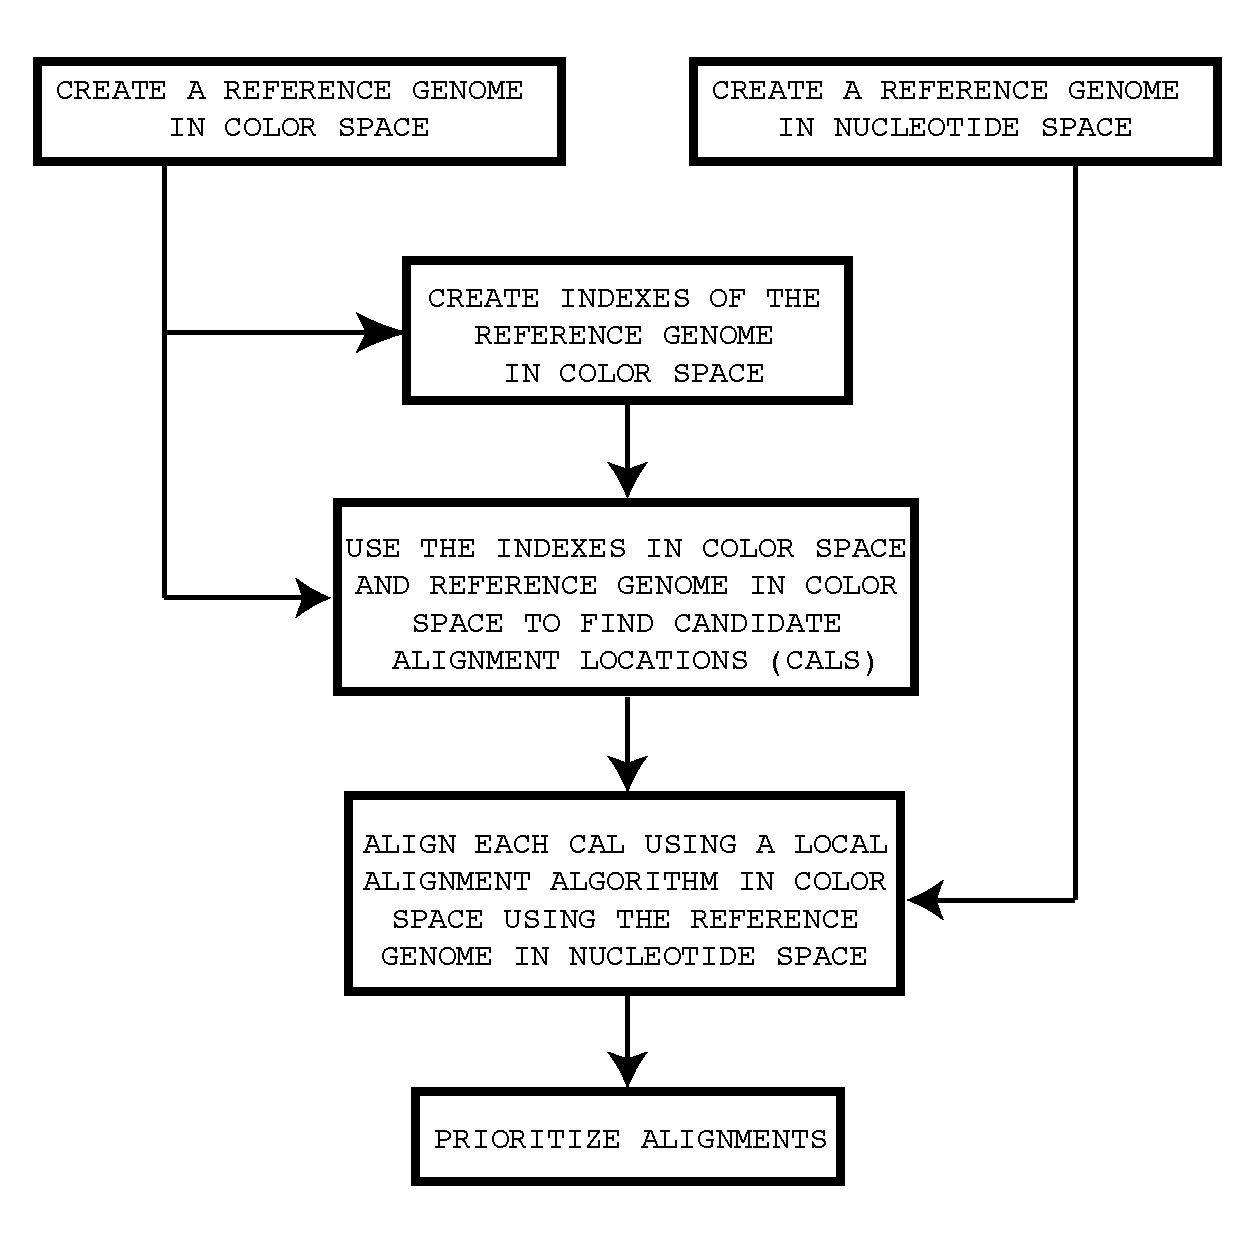
\includegraphics[scale=0.75]{work-flow-color.pdf}
	\caption{
	The BFAST work flow for color space alignment.
	}{
	See \autoref{sec:color-space-alignment} for a description.
	\label{fig:work-flow-color}
	}
\end{figure}
\chapter{Examples}
\section{Whole-Genome Alignment of Phi X 174}
\label{sec:phi}
In this example, we will align read to the Phi X 174 genome using the work flow presented in \autoref{sec:work-flow}.

To begin this example, open the URL: \url{http://bfast.soureforge.net}.
Under example datasets, right-click the file ``bfast-example-phi.x.174.tar.gz'' and select the ``save-as'' option to download the examples file.
To uncompress the compressed archive, in the command line type in ``tar zxvf bfast-example-phi.x.174.tar.gz'' (no quotes).

We first want to create a \BRGF{} (see \autoref{sec:fasta2brg}).
The \rGFF{} is stored in a file called ``phi.x.174.fa''.
The command we use to create the \BRGF{} is:
\begin{script}
	bfast fasta2brg -f phi.x.174.fa 
\end{script}
This should create a file called ``phi.x.174.fa.nt.brg'', which is the \BRGF{}.

The second step is to create the indexes using the \BRGF{} as input (see \autoref{sec:index}).
We will create five indexes that are chosen for $50$ base-pair reads, and robust against mismatches.
The method used to choose these indexes is not described here, but can be performed using \TT{btestindexes} (see \autoref{sec:btestindexes} and \autoref{sec:design-indexes}).
The commands we use to create the \BIF{s} is:
\begin{script}
	bfast index -f phi.x.174.fa -m 111111111111111111 -w 12 -i 1
	\\
	bfast index -f phi.x.174.fa -m 1111111110111111111 -w 12 -i 2
	\\
	bfast index -f phi.x.174.fa -m 111111011111101011111 -w 12 -i 3
	\\
	bfast index -f phi.x.174.fa -m 111111011001100111011111 -w 12 -i 4
	\\
	bfast index -f phi.x.174.fa -m 1111011101011111101111 -w 12 -i 5
\end{script}
This should create five files, one for each \BIF{}:
\begin{verbatim}
phi.x.174.fa.1.1.bif
phi.x.174.fa.2.1.bif
phi.x.174.fa.3.1.bif
phi.x.174.fa.4.1.bif
phi.x.174.fa.5.1.bif
\end{verbatim}

The third step is to find candidate alignment locations (CALs) for the set of reads using the indexes created in the second step (see \autoref{sec:match}).
We have generated synthetic reads from the Phi X 174 genome using \TT{bgeneratereads} (see \autoref{sec:bgeneratereads}).
We created reads with $0$ to $5$ mismatches, with $10,000$ reads created for each scenario, for a total of $60,000$ reads.
The reads file is ``reads.phi.x.174.fa''.
In this example we use all five indexes as our main indexes, and no secondary indexes.
We use all possible offsets, listed in ``offsets.txt''.
The command we use to find the matches is:
\begin{script}
	bfast match -f phi.x.174.fa -r reads.phi.x.174.fastq $>$  bfast.matches.file.phi.x.174.bmf
\end{script}
One file should be outputted, a \BMF{} (``bfast.matches.file.phi.x.174.bmf'').

The fourth step is to run the local alignment algorithm for each CAL for a given read (see \autoref{sec:localalign}).
The command we use to perform the local alignment is:
\begin{script}
	bfast localalign -f phi.x.174.fa -m bfast.matches.file.phi.x.174.bmf $>$ bfast.aligned.file.phi.x.174.baf
\end{script}
This should create one output file, a \BAF{} (``bfast.aligned.file.phi.x.174.baf'').

The fifth and final step is to prioritize the alignments (see \autoref{sec:postprocess}).
We use as input the \BAF{} created in the previous step.
In this case, we choose to output the best unambiguous alignment for each read.
The command we use to prioritize alignments is:
\begin{script}
	bfast postprocess -f phi.x.174.fa -i bfast.aligned.file.phi.x.174.baf $>$ bfast.reported.file.phi.x.174.sam
\end{script}
This should create one output file, a \BSAMF{}.

The third and fifth step can performed in a pipe-and-filter format, generating only one output file:
\begin{script}
	cat reads.phi.x.174.fastq $|$ bfast match -f phi.x.174.fa $|$ bfast localalign -f phi.x.174.fa $|$ bfast postprocess -f phi.x.174.fa $>$ bfast.reported.file.phi.x.174.sam
\end{script}
\chapter{Appendix}
\section{Human Genome Alignment Recommended Settings}
\label{sec:hg-settings}
We assume that you have the full hg18 reference in the FASTA format in a file called hg18.fa.
We detail our recommended commands to align sensitively to the human genome, at the cost of speed, outputting in the SAM format (see \url{http://samtools.sourceforge.net}).
Further filtering, especially filtering on mapping quality, alignment score, and alignment quality, should be also be performed.
For a more detailed explanation, please see \autoref{sec:phi}.
Please use the {\tt -n} option for multi-threaded alignment where possible.
For Illumina data see \autoref{sec:hg-settings-illumina}. 
For ABI SOLiD data see \autoref{sec:hg-settings-abi}

\subsection{Illumina}
\label{sec:hg-settings-illumina}
We assume your reads are in Illumina QSEQ format (the files that end with \_qseq.txt) and we wish to align lane $<N>$.
Note, we align one lane all at one time but splitting the converted reads file allows for parallelism.

We suggest a hash width of 14, although this should be reduced if you are splitting the indexes for low-memory computation.

For reads less than $>40$bp, the masks for the main indexes should be:\\
\\
\begin{boxedverbatim}
111111111111111111
111010001110001110100011011111
11110100110111101010101111
11111111111111001111
1111011101100101001111111
11110111000101010000010101110111
1011001101011110100110010010111
1110110010100001000101100111001111
1111011111111111111
11011111100010110111101101
\end{boxedverbatim}
\\
\\
For reads greater than or equal to $40$bp, the main indexes should be:\\
\begin{boxedverbatim}
1111111111111111111111
1111101110111010100101011011111
1011110101101001011000011010001111111
10111001101001100100111101010001011111
11111011011101111011111111
111111100101001000101111101110111
11110101110010100010101101010111111
111101101011011001100000101101001011101
1111011010001000110101100101100110100111
1111010010110110101110010110111011
\end{boxedverbatim}
\\

Given the above, the commands we should execute are:
\\\\
Convert the reads:\\
{\tt \scriptsize \$perl bfast-\Version{}/scripts/qseq2fastq.pl -q s\_<N>\\}
Convert the reference:\\
{\tt \scriptsize \$bfast-\Version{}/bfast/bfast fasta2brg -f hg18.fa\\}
Create the indexes:\\
{\tt \scriptsize \$bfast-\Version{}/bfast index -f hg18.fa -m <mask> -w 14 -i <index number>\\}
Search the indexes:\\
{\tt \scriptsize \$bfast-\Version{}/bfast match -f hg18.fa -r reads.s\_<N>.fastq $>$ bfast.matches.file.s\_<N>.bmf\\}
Perform local alignment:\\
{\tt \scriptsize \$bfast-\Version{}/bfast localalign -f hg18.fa -m bfast.matches.file.s\_<N>.bmf $>$ bfast.aligned.file.s\_<N>.baf\\}
Filter alignments:\\
{\tt \scriptsize \$bfast-\Version{}/bfast postprocess -f hg18.fa -i bfast.aligned.file.s\_<N>.baf\\
$>$ bfast.reported.file.s\_<N>.sam\\}
\\

\subsection{ABI SOLiD}
\label{sec:hg-settings-abi}
We assume your reads are at least $50$bp in length.
We will split the input into $10,000,000$ read pieces for parallel computation.

We suggest a hash width of 14, although this should be reduced if you are splitting the indexes for low-memory computation.

The masks for the main indexes should be:\\
\\
\begin{boxedverbatim}
1111111111111111111111
111110100111110011111111111
10111111011001100011111000111111
1111111100101111000001100011111011
111111110001111110011111111
11111011010011000011000110011111111
1111111111110011101111111
111011000011111111001111011111
1110110001011010011100101111101111
111111001000110001011100110001100011111
\end{boxedverbatim}
\\

Given the above files, the commands we should execute are:
\\\\
Convert the reads:\\
{\tt \scriptsize \$bfast-\Version{}/scripts/solid2fastq -n 10000000 -o reads *.csfasta *.qual\\}
Convert the reference (nucleotide space):\\
{\tt \scriptsize \$bfast-\Version{}/bfast fasta2brg -f hg18.fa\\}
Convert the reference (color space):\\
{\tt \scriptsize \$bfast-\Version{}/bfast fasta2brg -f hg18.fa -A 1 \\}
Create the indexes:\\
{\tt \scriptsize \$bfast-\Version{}/bfast index -f hg18.fa -m <mask> -w 14 -i <index number> -A 1\\}
Search the indexes:\\
{\tt \scriptsize \$bfast-\Version{}/bfast match -f hg18.fa -A 1 -r reads.<N>.fastq $>$ bfast.matches.file.hg18.<N>.bmf\\}
Perform local alignment:\\
{\tt \scriptsize \$bfast-\Version{}/bfast localalign -f hg18.fa -m bfast.matches.file.hg18.<N>.bmf -A \\
$>$ bfast.aligned.file.hg18.<N>.baf\\}
Filter alignments:\\
{\tt \scriptsize \$bfast-\Version{}/bfast postprocess -f hg18.fa -i bfast.aligned.file.hg18.<N>.baf -A 1\\
$>$ bfast.reported.file.hg18.<N>.sam\\}
\\
Note that for parallel computation, execute {\tt bfast match}, {\tt bfast localalign}, and {\tt bfast postprocess} for each converted input file created (replace $<N>$ with the input file number).
Also, since color space local alignment may be slower than the match step, we can use the \TT{-s} and \TT{-e} options in {\tt bfast localalign} to further parallelize the local alignment.

\section{High-Speed Tutorial}
\label{sec:high-speed-tutorial}
Not for the faint of heart, most details will be omitted.

Your best bet is to follow the work flow in \autoref{sec:work-flow} (or \autoref{sec:color-space-alignment} for color space).
A quick list of relevant sections are as follows:
\begin{itemize}
	\item Step 1: \autoref{sec:creating-a-rg}.
	\item Step 2: \autoref{sec:creating-bifs}.
	\item Step 3: \autoref{sec:finding-cals}.
	\item Step 4: \autoref{sec:local-alignment}.
	\item Step 5: \autoref{sec:prioritizing-alignments}.
\end{itemize}
\section{Copyright}
		    GNU GENERAL PUBLIC LICENSE
		       Version 2, June 1991

 Copyright (C) 1989, 1991 Free Software Foundation, Inc.,
 51 Franklin Street, Fifth Floor, Boston, MA 02110-1301 USA
 Everyone is permitted to copy and distribute verbatim copies
 of this license document, but changing it is not allowed.

			    Preamble

  The licenses for most software are designed to take away your
freedom to share and change it.  By contrast, the GNU General Public
License is intended to guarantee your freedom to share and change free
software--to make sure the software is free for all its users.  This
General Public License applies to most of the Free Software
Foundation's software and to any other program whose authors commit to
using it.  (Some other Free Software Foundation software is covered by
the GNU Lesser General Public License instead.)  You can apply it to
your programs, too.

  When we speak of free software, we are referring to freedom, not
price.  Our General Public Licenses are designed to make sure that you
have the freedom to distribute copies of free software (and charge for
this service if you wish), that you receive source code or can get it
if you want it, that you can change the software or use pieces of it
in new free programs; and that you know you can do these things.

  To protect your rights, we need to make restrictions that forbid
anyone to deny you these rights or to ask you to surrender the rights.
These restrictions translate to certain responsibilities for you if you
distribute copies of the software, or if you modify it.

  For example, if you distribute copies of such a program, whether
gratis or for a fee, you must give the recipients all the rights that
you have.  You must make sure that they, too, receive or can get the
source code.  And you must show them these terms so they know their
rights.

  We protect your rights with two steps: (1) copyright the software, and
(2) offer you this license which gives you legal permission to copy,
distribute and/or modify the software.

  Also, for each author's protection and ours, we want to make certain
that everyone understands that there is no warranty for this free
software.  If the software is modified by someone else and passed on, we
want its recipients to know that what they have is not the original, so
that any problems introduced by others will not reflect on the original
authors' reputations.

  Finally, any free program is threatened constantly by software
patents.  We wish to avoid the danger that redistributors of a free
program will individually obtain patent licenses, in effect making the
program proprietary.  To prevent this, we have made it clear that any
patent must be licensed for everyone's free use or not licensed at all.

  The precise terms and conditions for copying, distribution and
modification follow.

		    GNU GENERAL PUBLIC LICENSE
   TERMS AND CONDITIONS FOR COPYING, DISTRIBUTION AND MODIFICATION

  0. This License applies to any program or other work which contains
a notice placed by the copyright holder saying it may be distributed
under the terms of this General Public License.  The "Program", below,
refers to any such program or work, and a "work based on the Program"
means either the Program or any derivative work under copyright law:
that is to say, a work containing the Program or a portion of it,
either verbatim or with modifications and/or translated into another
language.  (Hereinafter, translation is included without limitation in
the term "modification".)  Each licensee is addressed as "you".

Activities other than copying, distribution and modification are not
covered by this License; they are outside its scope.  The act of
running the Program is not restricted, and the output from the Program
is covered only if its contents constitute a work based on the
Program (independent of having been made by running the Program).
Whether that is true depends on what the Program does.

  1. You may copy and distribute verbatim copies of the Program's
source code as you receive it, in any medium, provided that you
conspicuously and appropriately publish on each copy an appropriate
copyright notice and disclaimer of warranty; keep intact all the
notices that refer to this License and to the absence of any warranty;
and give any other recipients of the Program a copy of this License
along with the Program.

You may charge a fee for the physical act of transferring a copy, and
you may at your option offer warranty protection in exchange for a fee.

  2. You may modify your copy or copies of the Program or any portion
of it, thus forming a work based on the Program, and copy and
distribute such modifications or work under the terms of Section 1
above, provided that you also meet all of these conditions:

    a) You must cause the modified files to carry prominent notices
    stating that you changed the files and the date of any change.

    b) You must cause any work that you distribute or publish, that in
    whole or in part contains or is derived from the Program or any
    part thereof, to be licensed as a whole at no charge to all third
    parties under the terms of this License.

    c) If the modified program normally reads commands interactively
    when run, you must cause it, when started running for such
    interactive use in the most ordinary way, to print or display an
    announcement including an appropriate copyright notice and a
    notice that there is no warranty (or else, saying that you provide
    a warranty) and that users may redistribute the program under
    these conditions, and telling the user how to view a copy of this
    License.  (Exception: if the Program itself is interactive but
    does not normally print such an announcement, your work based on
    the Program is not required to print an announcement.)

These requirements apply to the modified work as a whole.  If
identifiable sections of that work are not derived from the Program,
and can be reasonably considered independent and separate works in
themselves, then this License, and its terms, do not apply to those
sections when you distribute them as separate works.  But when you
distribute the same sections as part of a whole which is a work based
on the Program, the distribution of the whole must be on the terms of
this License, whose permissions for other licensees extend to the
entire whole, and thus to each and every part regardless of who wrote it.

Thus, it is not the intent of this section to claim rights or contest
your rights to work written entirely by you; rather, the intent is to
exercise the right to control the distribution of derivative or
collective works based on the Program.

In addition, mere aggregation of another work not based on the Program
with the Program (or with a work based on the Program) on a volume of
a storage or distribution medium does not bring the other work under
the scope of this License.

  3. You may copy and distribute the Program (or a work based on it,
under Section 2) in object code or executable form under the terms of
Sections 1 and 2 above provided that you also do one of the following:

    a) Accompany it with the complete corresponding machine-readable
    source code, which must be distributed under the terms of Sections
    1 and 2 above on a medium customarily used for software interchange; or,

    b) Accompany it with a written offer, valid for at least three
    years, to give any third party, for a charge no more than your
    cost of physically performing source distribution, a complete
    machine-readable copy of the corresponding source code, to be
    distributed under the terms of Sections 1 and 2 above on a medium
    customarily used for software interchange; or,

    c) Accompany it with the information you received as to the offer
    to distribute corresponding source code.  (This alternative is
    allowed only for noncommercial distribution and only if you
    received the program in object code or executable form with such
    an offer, in accord with Subsection b above.)

The source code for a work means the preferred form of the work for
making modifications to it.  For an executable work, complete source
code means all the source code for all modules it contains, plus any
associated interface definition files, plus the scripts used to
control compilation and installation of the executable.  However, as a
special exception, the source code distributed need not include
anything that is normally distributed (in either source or binary
form) with the major components (compiler, kernel, and so on) of the
operating system on which the executable runs, unless that component
itself accompanies the executable.

If distribution of executable or object code is made by offering
access to copy from a designated place, then offering equivalent
access to copy the source code from the same place counts as
distribution of the source code, even though third parties are not
compelled to copy the source along with the object code.

  4. You may not copy, modify, sublicense, or distribute the Program
except as expressly provided under this License.  Any attempt
otherwise to copy, modify, sublicense or distribute the Program is
void, and will automatically terminate your rights under this License.
However, parties who have received copies, or rights, from you under
this License will not have their licenses terminated so long as such
parties remain in full compliance.

  5. You are not required to accept this License, since you have not
signed it.  However, nothing else grants you permission to modify or
distribute the Program or its derivative works.  These actions are
prohibited by law if you do not accept this License.  Therefore, by
modifying or distributing the Program (or any work based on the
Program), you indicate your acceptance of this License to do so, and
all its terms and conditions for copying, distributing or modifying
the Program or works based on it.

  6. Each time you redistribute the Program (or any work based on the
Program), the recipient automatically receives a license from the
original licensor to copy, distribute or modify the Program subject to
these terms and conditions.  You may not impose any further
restrictions on the recipients' exercise of the rights granted herein.
You are not responsible for enforcing compliance by third parties to
this License.

  7. If, as a consequence of a court judgment or allegation of patent
infringement or for any other reason (not limited to patent issues),
conditions are imposed on you (whether by court order, agreement or
otherwise) that contradict the conditions of this License, they do not
excuse you from the conditions of this License.  If you cannot
distribute so as to satisfy simultaneously your obligations under this
License and any other pertinent obligations, then as a consequence you
may not distribute the Program at all.  For example, if a patent
license would not permit royalty-free redistribution of the Program by
all those who receive copies directly or indirectly through you, then
the only way you could satisfy both it and this License would be to
refrain entirely from distribution of the Program.

If any portion of this section is held invalid or unenforceable under
any particular circumstance, the balance of the section is intended to
apply and the section as a whole is intended to apply in other
circumstances.

It is not the purpose of this section to induce you to infringe any
patents or other property right claims or to contest validity of any
such claims; this section has the sole purpose of protecting the
integrity of the free software distribution system, which is
implemented by public license practices.  Many people have made
generous contributions to the wide range of software distributed
through that system in reliance on consistent application of that
system; it is up to the author/donor to decide if he or she is willing
to distribute software through any other system and a licensee cannot
impose that choice.

This section is intended to make thoroughly clear what is believed to
be a consequence of the rest of this License.

  8. If the distribution and/or use of the Program is restricted in
certain countries either by patents or by copyrighted interfaces, the
original copyright holder who places the Program under this License
may add an explicit geographical distribution limitation excluding
those countries, so that distribution is permitted only in or among
countries not thus excluded.  In such case, this License incorporates
the limitation as if written in the body of this License.

  9. The Free Software Foundation may publish revised and/or new versions
of the General Public License from time to time.  Such new versions will
be similar in spirit to the present version, but may differ in detail to
address new problems or concerns.

Each version is given a distinguishing version number.  If the Program
specifies a version number of this License which applies to it and "any
later version", you have the option of following the terms and conditions
either of that version or of any later version published by the Free
Software Foundation.  If the Program does not specify a version number of
this License, you may choose any version ever published by the Free Software
Foundation.

  10. If you wish to incorporate parts of the Program into other free
programs whose distribution conditions are different, write to the author
to ask for permission.  For software which is copyrighted by the Free
Software Foundation, write to the Free Software Foundation; we sometimes
make exceptions for this.  Our decision will be guided by the two goals
of preserving the free status of all derivatives of our free software and
of promoting the sharing and reuse of software generally.

			    NO WARRANTY

  11. BECAUSE THE PROGRAM IS LICENSED FREE OF CHARGE, THERE IS NO WARRANTY
FOR THE PROGRAM, TO THE EXTENT PERMITTED BY APPLICABLE LAW.  EXCEPT WHEN
OTHERWISE STATED IN WRITING THE COPYRIGHT HOLDERS AND/OR OTHER PARTIES
PROVIDE THE PROGRAM "AS IS" WITHOUT WARRANTY OF ANY KIND, EITHER EXPRESSED
OR IMPLIED, INCLUDING, BUT NOT LIMITED TO, THE IMPLIED WARRANTIES OF
MERCHANTABILITY AND FITNESS FOR A PARTICULAR PURPOSE.  THE ENTIRE RISK AS
TO THE QUALITY AND PERFORMANCE OF THE PROGRAM IS WITH YOU.  SHOULD THE
PROGRAM PROVE DEFECTIVE, YOU ASSUME THE COST OF ALL NECESSARY SERVICING,
REPAIR OR CORRECTION.

  12. IN NO EVENT UNLESS REQUIRED BY APPLICABLE LAW OR AGREED TO IN WRITING
WILL ANY COPYRIGHT HOLDER, OR ANY OTHER PARTY WHO MAY MODIFY AND/OR
REDISTRIBUTE THE PROGRAM AS PERMITTED ABOVE, BE LIABLE TO YOU FOR DAMAGES,
INCLUDING ANY GENERAL, SPECIAL, INCIDENTAL OR CONSEQUENTIAL DAMAGES ARISING
OUT OF THE USE OR INABILITY TO USE THE PROGRAM (INCLUDING BUT NOT LIMITED
TO LOSS OF DATA OR DATA BEING RENDERED INACCURATE OR LOSSES SUSTAINED BY
YOU OR THIRD PARTIES OR A FAILURE OF THE PROGRAM TO OPERATE WITH ANY OTHER
PROGRAMS), EVEN IF SUCH HOLDER OR OTHER PARTY HAS BEEN ADVISED OF THE
POSSIBILITY OF SUCH DAMAGES.

		     END OF TERMS AND CONDITIONS

	    How to Apply These Terms to Your New Programs

  If you develop a new program, and you want it to be of the greatest
possible use to the public, the best way to achieve this is to make it
free software which everyone can redistribute and change under these terms.

  To do so, attach the following notices to the program.  It is safest
to attach them to the start of each source file to most effectively
convey the exclusion of warranty; and each file should have at least
the "copyright" line and a pointer to where the full notice is found.

    <one line to give the program's name and a brief idea of what it does.>
    Copyright (C) <year>  <name of author>

    This program is free software; you can redistribute it and/or modify
    it under the terms of the GNU General Public License as published by
    the Free Software Foundation; either version 2 of the License, or
    (at your option) any later version.

    This program is distributed in the hope that it will be useful,
    but WITHOUT ANY WARRANTY; without even the implied warranty of
    MERCHANTABILITY or FITNESS FOR A PARTICULAR PURPOSE.  See the
    GNU General Public License for more details.

    You should have received a copy of the GNU General Public License along
    with this program; if not, write to the Free Software Foundation, Inc.,
    51 Franklin Street, Fifth Floor, Boston, MA 02110-1301 USA.

Also add information on how to contact you by electronic and paper mail.

If the program is interactive, make it output a short notice like this
when it starts in an interactive mode:

    Gnomovision version 69, Copyright (C) year name of author
    Gnomovision comes with ABSOLUTELY NO WARRANTY; for details type `show w'.
    This is free software, and you are welcome to redistribute it
    under certain conditions; type `show c' for details.

The hypothetical commands `show w' and `show c' should show the appropriate
parts of the General Public License.  Of course, the commands you use may
be called something other than `show w' and `show c'; they could even be
mouse-clicks or menu items--whatever suits your program.

You should also get your employer (if you work as a programmer) or your
school, if any, to sign a "copyright disclaimer" for the program, if
necessary.  Here is a sample; alter the names:

  Yoyodyne, Inc., hereby disclaims all copyright interest in the program
  `Gnomovision' (which makes passes at compilers) written by James Hacker.

  <signature of Ty Coon>, 1 April 1989
  Ty Coon, President of Vice

This General Public License does not permit incorporating your program into
proprietary programs.  If your program is a subroutine library, you may
consider it more useful to permit linking proprietary applications with the
library.  If this is what you want to do, use the GNU Lesser General
Public License instead of this License.


% References
\phantomsection
\addcontentsline{toc}{chapter}{References}
\bibliography{bfast-book}
\bibliographystyle{natbib}
\end{document}
